\documentclass{elsarticle}
\usepackage{amsmath,amssymb}
\usepackage{graphicx}
\usepackage{float}
\usepackage{booktabs}
\usepackage{multirow}
\usepackage{hyperref}
\usepackage{float}
\usepackage[numbers]{natbib}

\begin{document}

\title{A CFD-Informed Surrogate for Rapid Flow Prediction in an Argon-Stirred Ladle: VOF-Based Domain Decomposition, Cross-Position Generalization, and Multi-Baseline Benchmarking}

\author[shu]{Yiming Liu}
\author[shu]{Wentao Zhang}
\author[shu]{Xutong Wang}
\author[shu]{Guangxin Wu\corref{corresponding}}
\cortext[corresponding]{Corresponding author. E-mail: gxwu@shu.edu.cn}
\address[shu]{School of Materials Science and Engineering \& State Key Laboratory of Advanced Special Steel, Shanghai University, Shanghai 200444, PR China}

\begin{abstract}
Repeated CFD simulations of argon-stirred ladle flow are computationally prohibitive when multiple operating conditions must be evaluated. This study develops a CFD-informed surrogate combining volume-of-fluid (VOF)-based domain decomposition with neural network regression for rapid prediction of the statistically steady liquid-steel flow field under varying gas flow rates ($Q$) and injection positions ($m$). The key insight is that restricting the learning problem to the steel phase---where the three-phase VOF equations reduce rigorously to single-phase incompressible RANS---eliminates ill-conditioned multiphase residuals without requiring interface boundary conditions. An $8\times384$ SiLU multilayer perceptron trained on VOF-filtered steel-phase data achieves $R^{2}=0.983$ for center-blowing with near-zero extrapolation degradation. A binary injection-position parameter $m\in\{0,1\}$ enables cross-position generalization: joint training recovers $R^{2}=0.94$--$0.97$ for eccentric-blowing, whereas a center-only model collapses ($R^{2}<0$). Six baselines are compared. Proper orthogonal decomposition (POD-ROM) achieves the highest center-blowing accuracy ($R^{2}=0.994$) with only two spatial modes, confirming the low-rank nature of $Q$-dependent flow variation. However, POD modes are tied to a specific spatial structure and fail completely across injection positions ($R^{2}<0$). The proposed surrogate replaces two separate POD models with a single network, predicting the full three-dimensional field in $\sim$5 seconds per operating condition.
\end{abstract}

\begin{keyword}
CFD; Surrogate modeling; Ladle furnace; VOF; Cross-position generalization; POD-ROM; Neural network
\end{keyword}

\maketitle

\section{Introduction}

Ladle furnace (LF) refining is critical for controlling steel cleanliness, thermal uniformity, and compositional homogeneity \cite{liu2026cfd}. During bottom argon stirring, the injected gas forms a buoyancy-driven plume that induces strong recirculation \cite{mazumdar1995physical}, enhancing mixing and promoting inclusion transport \cite{li2020numerical}. Excessively strong stirring may expose steel through slag eye formation, increasing re-oxidation risk \cite{jonsson1996modeling}. Reliable flow-field prediction is therefore fundamental to process optimization.

CFD coupled with VOF and DPM has become a standard tool for ladle hydrodynamics \cite{liu2019numerical,ersson2008fluid,cloete2010mathematical}. A companion CFD study by the present authors \cite{liu2026cfd} employs the same VOF-DPM framework---molten steel, slag, and top air resolved via Eulerian VOF, argon bubbles tracked as Lagrangian DPM particles---applied to the same 40-ton gas-stirred ladle geometry across five argon flow rates (40--120 NL/min). However, high-fidelity multiphase simulations require upwards of 36 hours per case, making multi-condition evaluation prohibitive. Machine learning surrogates provide predictions orders of magnitude faster \cite{brunton2020machine}. Physics-informed neural networks (PINNs) incorporate governing-equation residuals into training \cite{raissi2019physics,karniadakis2021physics}, with applications across fluid mechanics \cite{cai2021physics,cuomo2022scientific}. Challenges include training instability \cite{wang2021understanding} and multiphase interface handling \cite{jin2021nsfnet}.

A key challenge for ladle-flow surrogates is the three-phase system spanning four orders of magnitude in density. Enforcing Navier--Stokes residuals across the entire domain is ill-conditioned. We propose a VOF-based domain decomposition: in pure-steel cells ($\alpha_{\rm steel}\to 1$), the VOF mixture equations reduce to single-phase incompressible RANS. Rather than solving multiphase equations within the network, we restrict the learning problem to the steel phase through VOF filtering. A binary injection-position parameter $m\in\{0,1\}$ enables a single surrogate for both center-bottom and eccentric-bottom blowing.

Projection-based reduced-order models such as POD-ROM \cite{benner2015survey} offer an alternative surrogate paradigm, decomposing the flow field into spatial modes and interpolating mode coefficients across operating conditions. While effective for single-configuration problems, POD modes are tied to a specific spatial structure and cannot generalize across injection positions.

Contributions: (1) VOF-based domain decomposition that restricts learning to the steel phase; (2) $m$ parameterization enabling cross-position generalization with a single model; (3) six-baseline comparison including POD-ROM; (4) demonstration that POD fails across injection positions while the proposed surrogate succeeds; (5) surrogate achieving $R^{2}=0.983$ with 5-second inference.

\section{CFD Model}

\subsection{Geometry and Computational Domain}
The ladle was modeled as a truncated cone (Table~\ref{tab:geometry}), identical to the configuration used in the companion CFD study \cite{liu2026cfd}. Argon is introduced through a bottom nozzle at the center ($m=0$) or at one-third radius ($m=1$, $x\approx 0.47$ m). DPM treats argon bubbles as Lagrangian particles exchanging momentum with the continuous phase through drag forces.

\begin{table}[h]
\centering
\caption{Main dimensions.}
\label{tab:geometry}
\begin{tabular}{lc}
\toprule Parameter & Value \\ \midrule
Upper / lower diameter & 2.077 / 1.832 m \\
Steel + slag height & 1.85 m \\
Slag thickness & 0.15 m \\
Nozzle diameter & 0.08 m \\
Eccentric nozzle position & $(0.47, 0, 0)$ \\
\bottomrule
\end{tabular}
\end{table}

\subsection{Mesh and Turbulence Modeling}
An unstructured mesh with $9.32\times 10^{5}$ cells (Table~\ref{tab:mesh}) and realizable $k$--$\varepsilon$ turbulence model \cite{shih1995new} were used.

\begin{table}[h]
\centering
\caption{Mesh-independence.}
\label{tab:mesh}
\begin{tabular}{lccc}
\toprule Level & Cells & $|U|_{\max}$ (m/s) & Diff. (\%) \\ \midrule
Coarse  & 612,450  & 0.392 & 10.09 \\
Medium  & 932,080  & 0.431 & 1.40 \\
Fine    & 1,356,740 & 0.436 & --- \\
\bottomrule
\end{tabular}
\end{table}

\subsection{Dataset and Quality Verification}
Five center-blowing ($Q=40$--$120$ NL/min) and three eccentric-blowing ($Q=40,80,120$ NL/min) CFD cases were exported as 12-column CSV. All eight datasets satisfy $\sum\alpha_i\equiv 1$ (100\% verification). Velocity monotonicity: 18 layers $\times$ 5Q, zero violations (Table~\ref{tab:mono}).

\begin{table}[h]
\centering
\caption{Velocity monotonicity: mean $|\mathbf{U}|$ (m/s).}
\label{tab:mono}
\small
\begin{tabular}{lccccc}
\toprule $z$ (m) & $Q=40$ & $Q=60$ & $Q=80$ & $Q=100$ & $Q=120$ \\ \midrule
0.5 & 0.009 & 0.010 & 0.011 & 0.012 & 0.014 \\
1.0 & 0.017 & 0.022 & 0.025 & 0.027 & 0.031 \\
1.5 & 0.027 & 0.033 & 0.037 & 0.039 & 0.043 \\
1.8 & 0.044 & 0.053 & 0.059 & 0.063 & 0.069 \\
\bottomrule
\end{tabular}
\end{table}

\section{Methodology}

\begin{figure}[H]
\centering
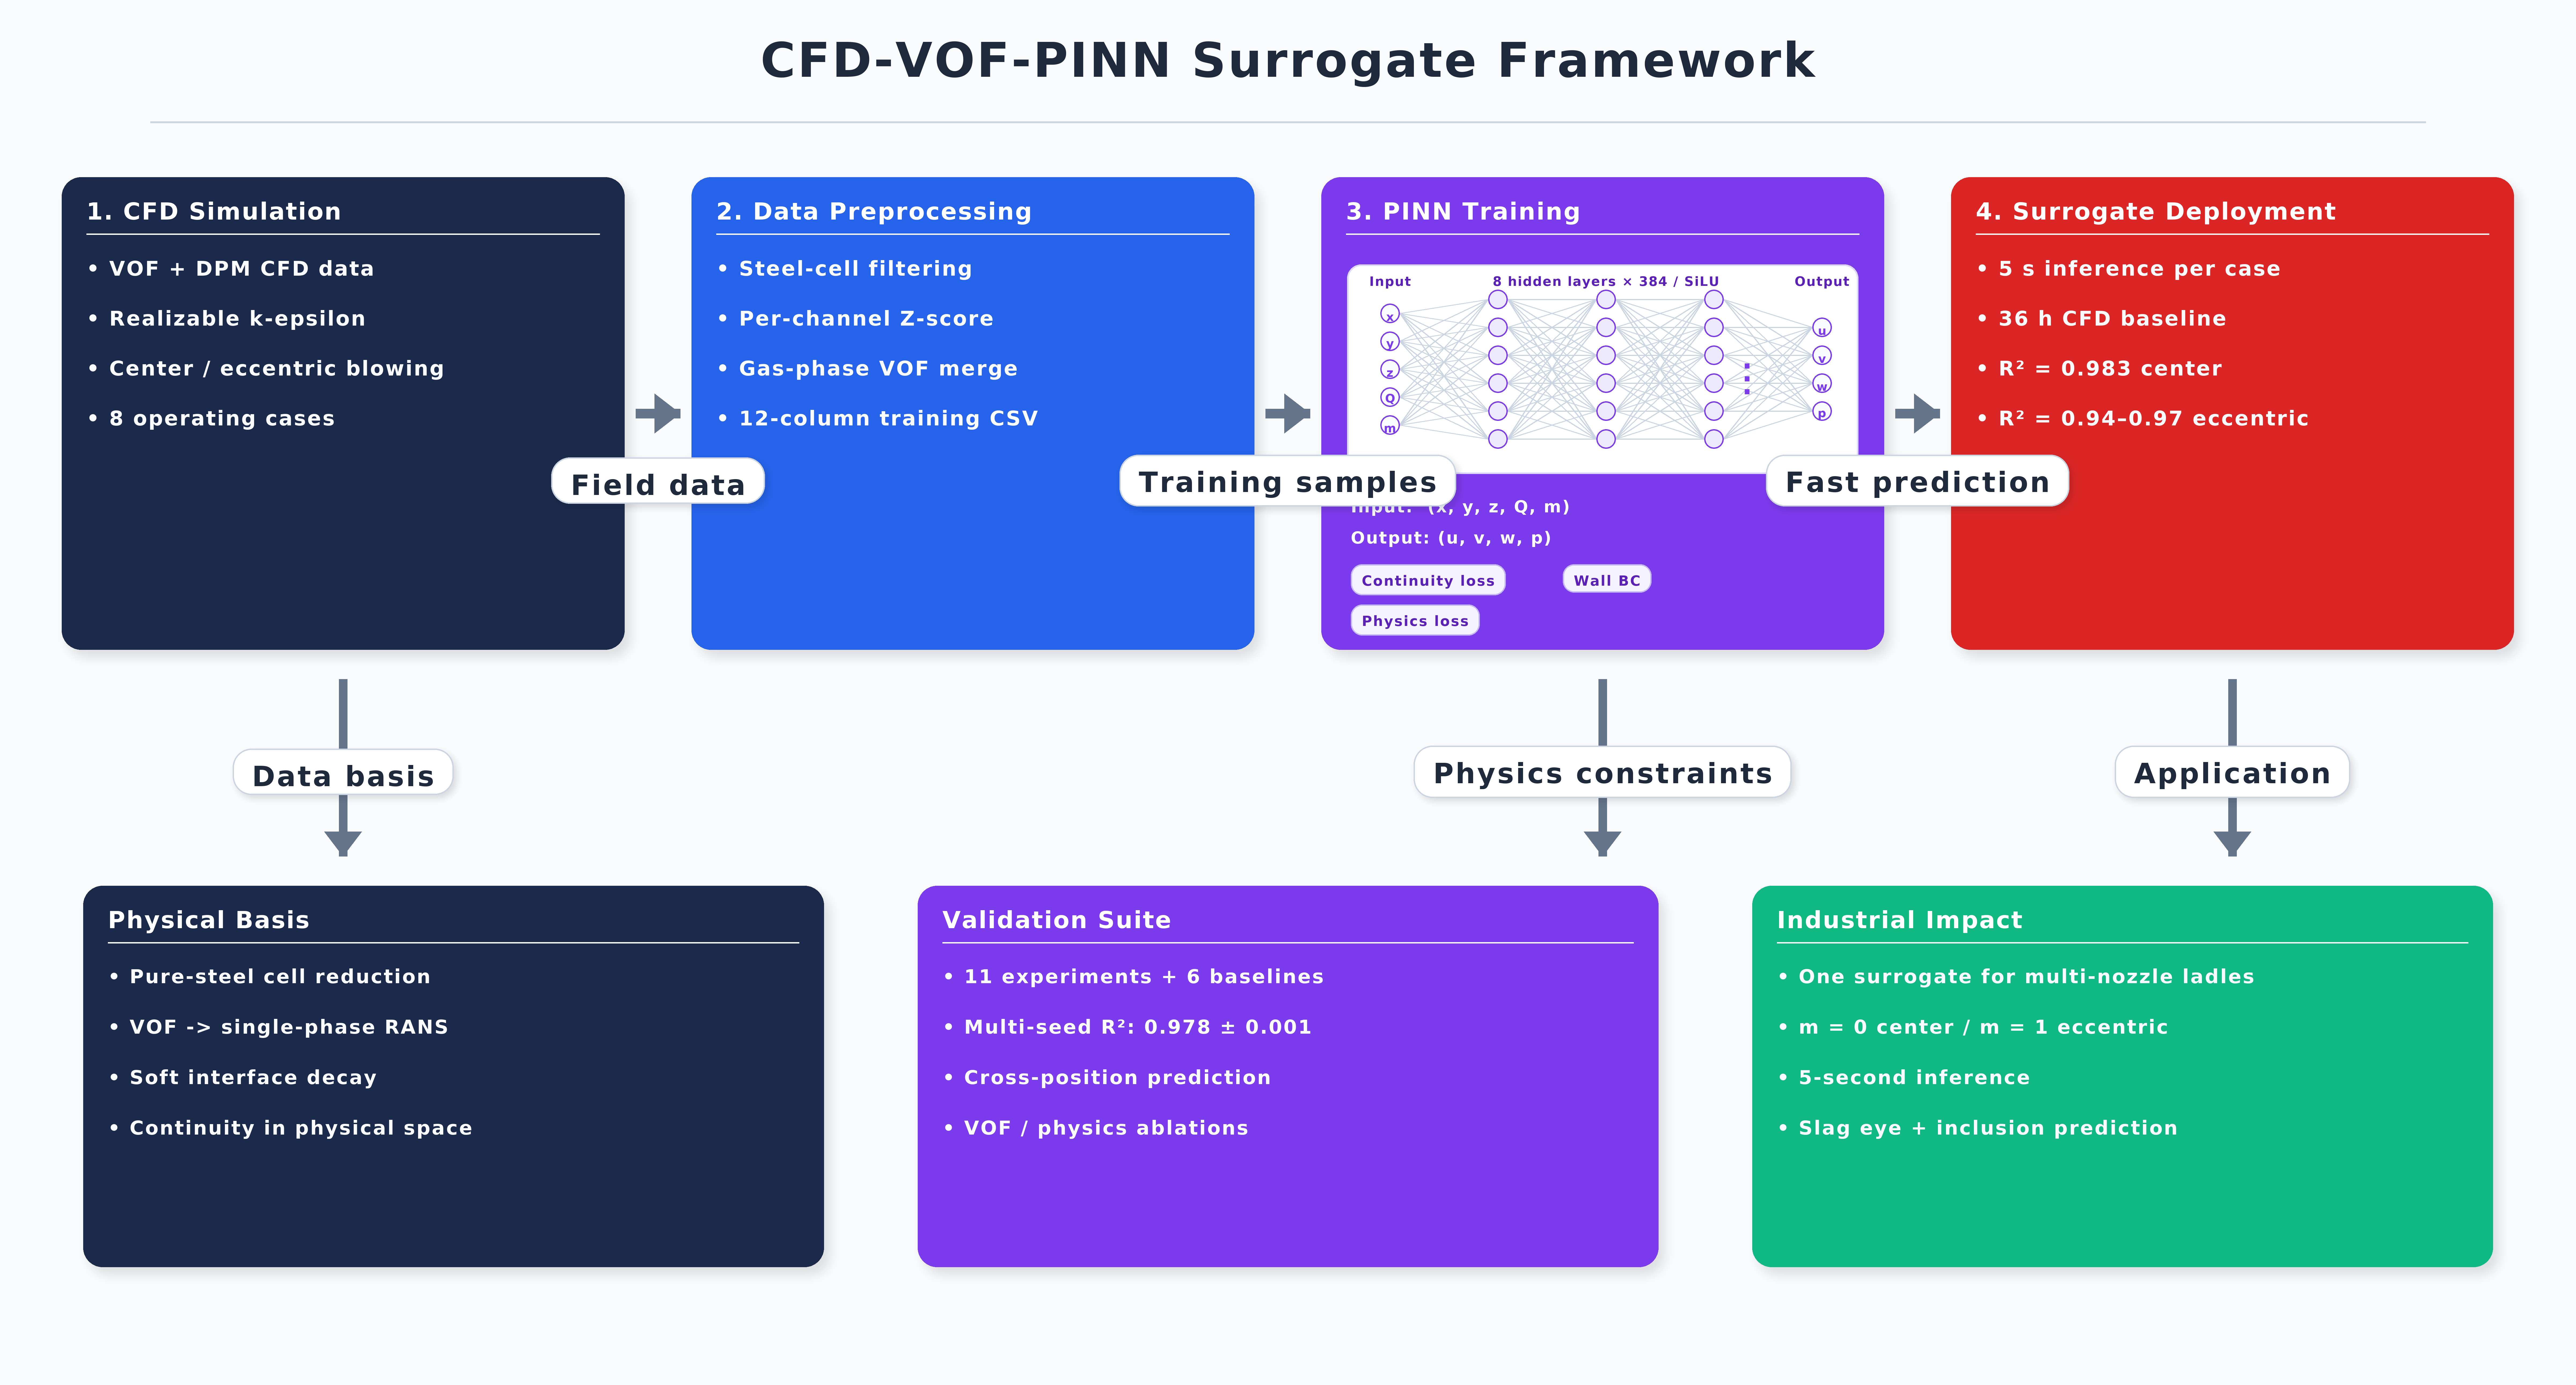
\includegraphics[width=\textwidth]{figures/fig1_framework.png}
\caption{Overview of the proposed CFD-informed surrogate framework.}
\label{fig:framework}
\end{figure}

\subsection{VOF-Based Domain Decomposition}
The central idea is to restrict the learning problem to the steel phase. In pure-steel cells ($\alpha_{\rm steel}\to 1$): $\rho\to\rho_{\rm steel}$, $\mu\to\mu_{\rm steel}$, $\mathbf{F}_{\sigma}\to 0$, and the VOF mixture equations reduce to single-phase incompressible RANS. Rather than solving multiphase equations within the network---which would be ill-conditioned across a four-order-of-magnitude density range---we simply filter the training data to $\alpha_{\rm steel}>0.01$. This filter eliminates slag and gas cells where the mixture momentum balance is ill-defined.

For physics-informed training, a soft spatial decay function deactivates continuity constraints near the interface:
$w_{\rm pde}=w_{\rm data}\cdot 0.5[1+\cos(\pi\cdot\min((z_{\rm top}-z)/T,1))]$
with $z_{\rm top}=1.85$ m, $T=0.20$ m. However, as shown in Section~\ref{sec:results_physics}, the continuity constraint provides only a marginal gain ($+0.014$ $R^{2}$) and the best model does not use it---filtering alone accounts for the dominant performance improvement.

\begin{table}[h]
\centering
\caption{Verified phase stratification (mean VOF).}
\label{tab:vof_strat}
\begin{tabular}{lccc}
\toprule $z$ (m) & $\bar{\alpha}_{\rm steel}$ & $\bar{\alpha}_{\rm slag}$ & $\bar{\alpha}_{\rm argon}$ \\ \midrule
0--1.6   & 1.000 & 0.000 & 0.000 \\
1.6--1.85 & 0.731 & 0.269 & 0.000 \\
1.85--2.05 & 0.000 & 0.701 & 0.299 \\
2.05--2.55 & 0.000 & 0.000 & 1.000 \\
\bottomrule
\end{tabular}
\end{table}

\begin{figure}[H]
\centering
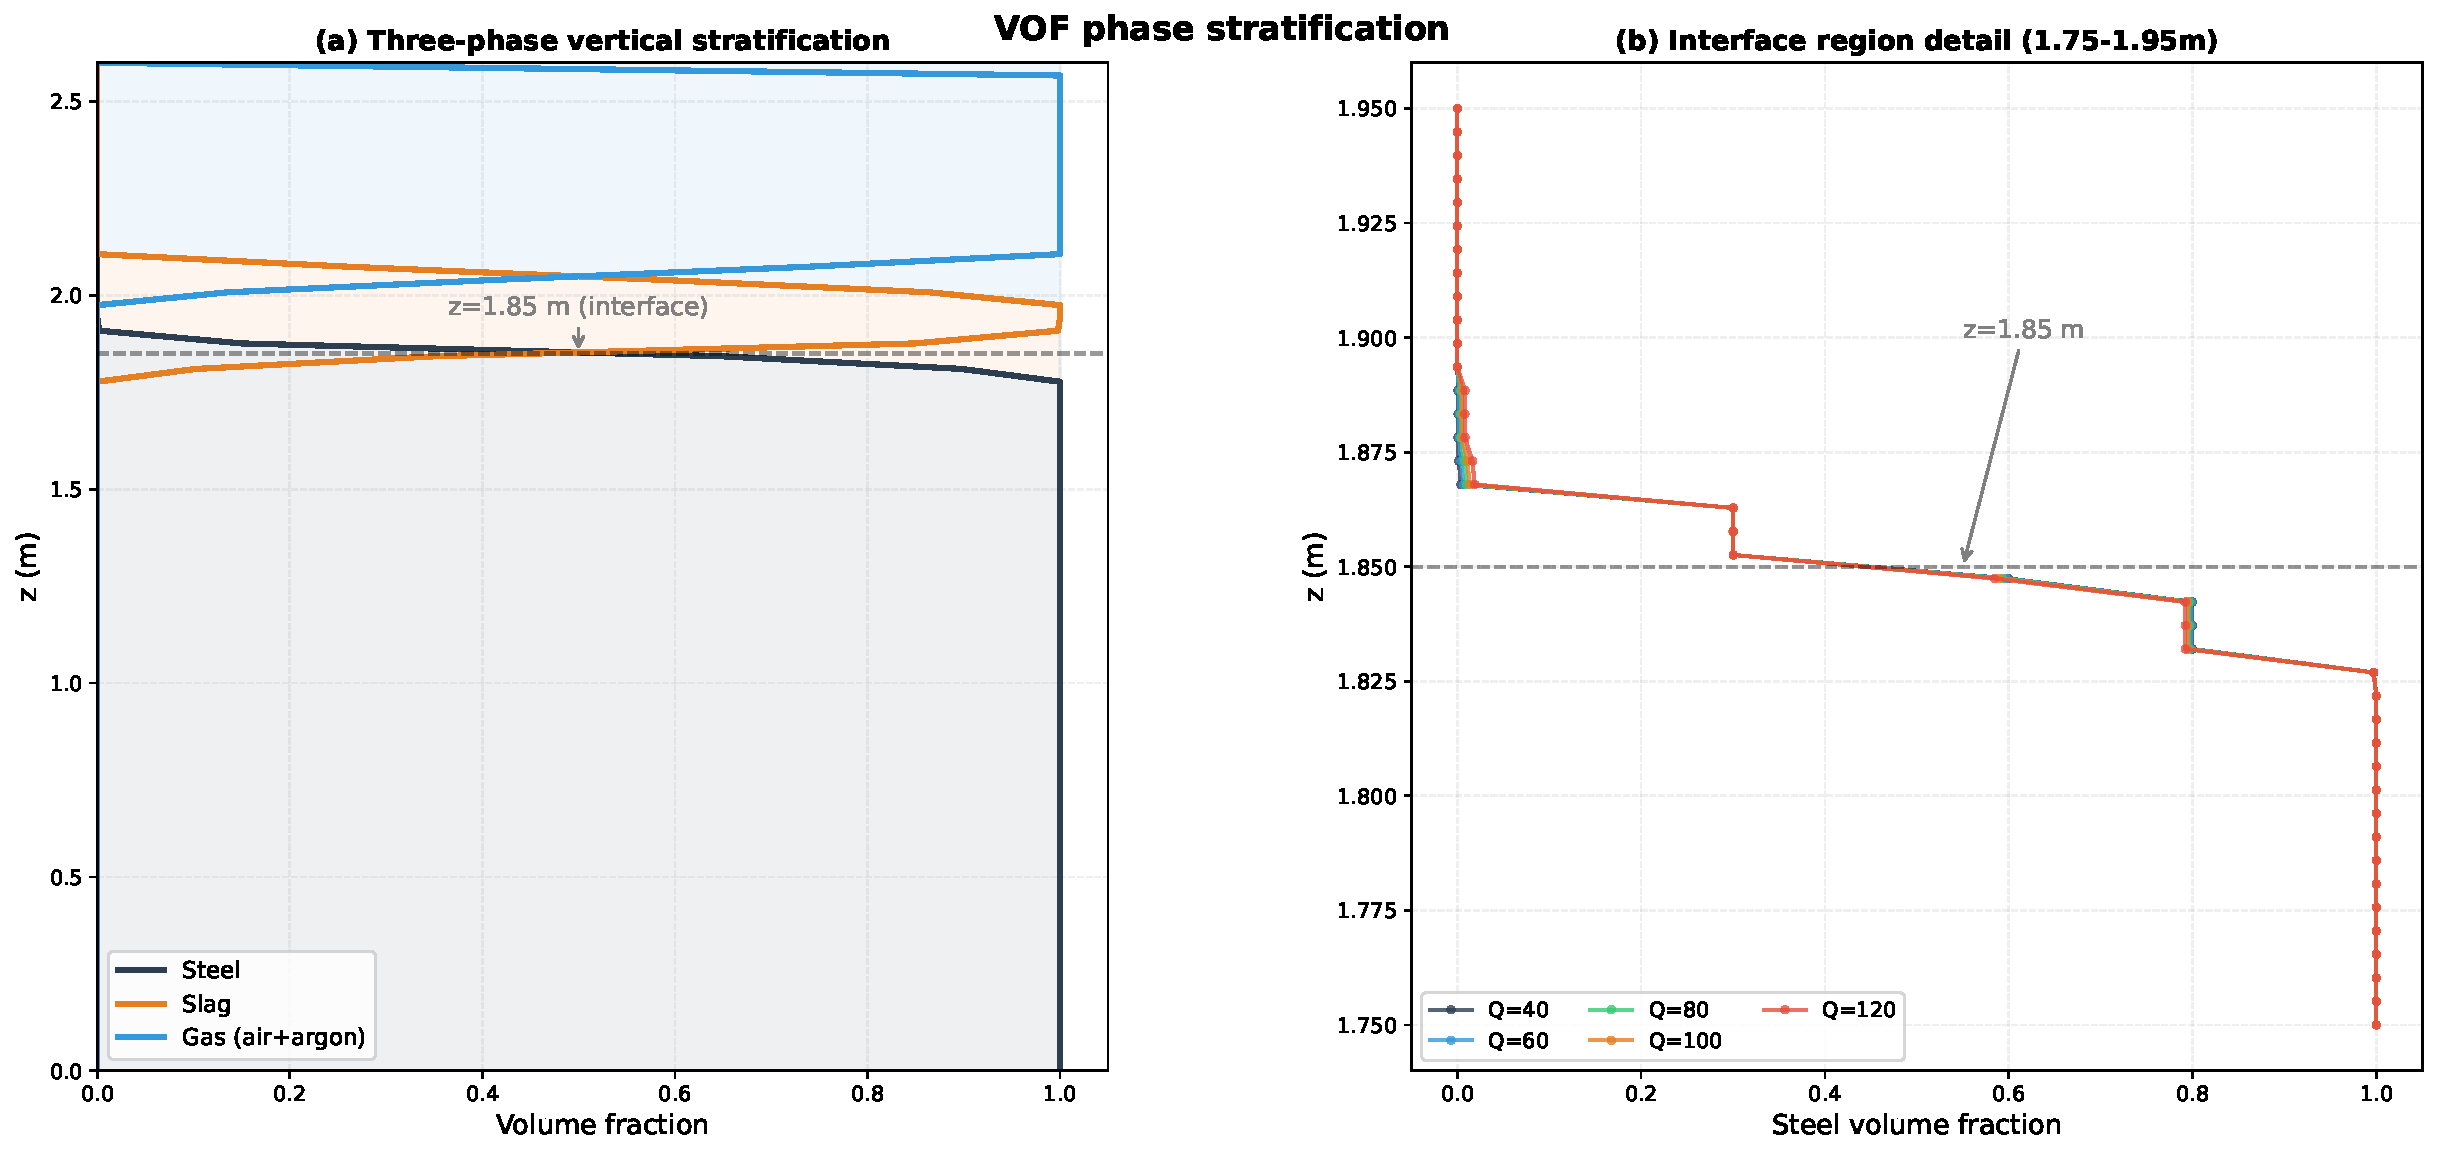
\includegraphics[width=\textwidth]{figures/fig2_vof_stratification.pdf}
\caption{Three-phase stratification. (a) Steel, slag, and argon profiles---identical across $Q$. (b) Interface detail.}
\label{fig:vof}
\end{figure}

\subsection{Network Architecture and Training}
The model maps $(x,y,z,Q,m)$ to $(\hat{u},\hat{v},\hat{w},\hat{p})$ via an $8\times 384$ SiLU MLP (1.04M parameters). Outputs use z-score normalization per channel. For ablation studies, a $6\times 128$ variant (84K parameters) is used. A continuity residual $\mathcal{R}_{\rm cont}=\nabla\cdot\mathbf{u}$ evaluated in physical space is available as an optional regularization term. Wall no-slip is enforced on steel-region boundary points ($\sim$42K points). Training: Adam (lr $=10^{-3}$), batch 8192, 2500 epochs, RTX 5070 GPU ($\sim$5 min). Inference: $\sim$5 s for $9.3\times 10^{5}$ cells.

\subsection{POD-ROM Baseline}
POD-ROM was implemented as a comparative baseline. Velocity magnitude snapshots from three training cases ($Q=40,60,80$ NL/min) form a snapshot matrix $\mathbf{X}\in\mathbb{R}^{3\times N}$ where $N=932{,}079$. SVD of the centered matrix yields two spatial modes capturing 100\% of snapshot variance. Mode coefficients are interpolated to test $Q$ values via thin-plate-spline RBF. Due to the smooth $Q$-dependence of the flow field, this approach achieves near-perfect reconstruction. However, because POD modes are tied to the spatial structure of a specific injection configuration, the model cannot generalize across positions---a limitation demonstrated in Section~\ref{sec:results_cross}.

\section{Experimental Setup}
Training: center-blowing $Q=40,60,80$ NL/min. Extrapolation testing: center-blowing $Q=100,120$ NL/min. Cross-position testing: eccentric-blowing $Q=40,80,120$ NL/min ($m=1$). Six baselines: POD-ROM, MLP $8\times384$, MLP $6\times128$, DeepONet ($p=50$), Kriging GPR (2000 inducing points), KAN. Metrics: $R^{2}$ on velocity magnitude, per-field $R^{2}$, multi-seed ensemble stability.

\section{Results}

\subsection{VOF Stratification and Centerline Validation}
Three-phase stratification is identical across all five $Q$ values (Fig.~\ref{fig:vof}), confirming consistent CFD setup. Centerline velocity profiles (Fig.~\ref{fig:centerline}) show close agreement for all eight configurations; relative errors remain below 10\% through most of the domain.

\begin{figure}[H]
\centering
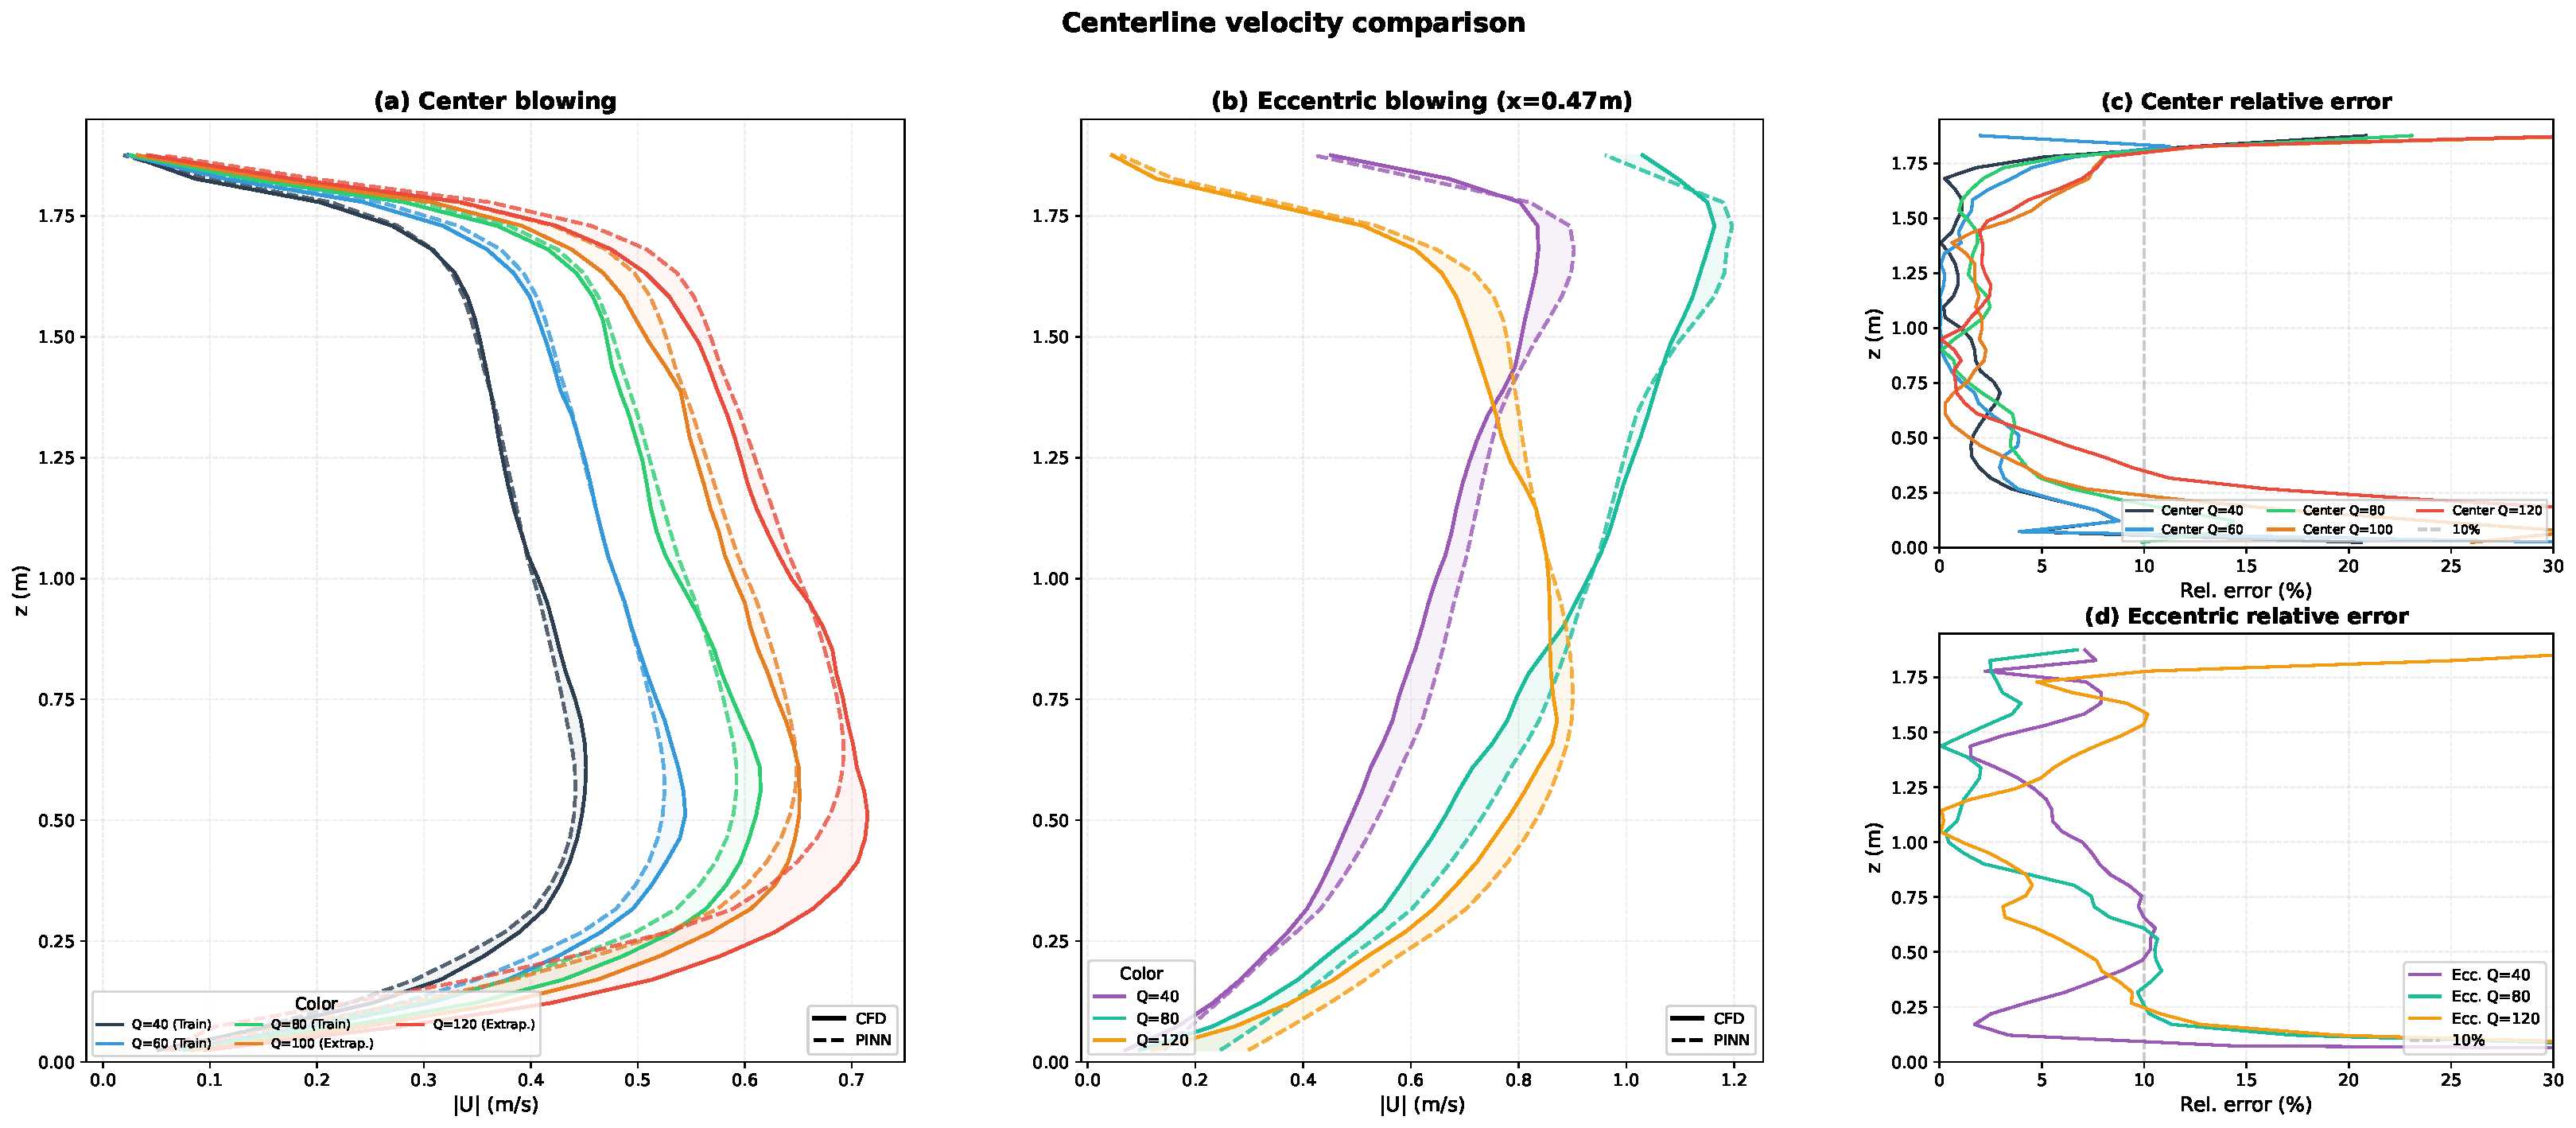
\includegraphics[width=\textwidth]{figures/fig_centerline_combined.pdf}
\caption{Centerline velocity: (a) center-blowing, (b) eccentric-blowing, (c) center relative error, (d) eccentric relative error. Solid: CFD; dashed: prediction.}
\label{fig:centerline}
\end{figure}

\subsection{Physics Ablation and Baseline Comparison}
\label{sec:results_physics}
Physics term ablation (Fig.~\ref{fig:abl_base}a) shows that the continuity constraint provides a modest $+0.014$ $R^{2}$ improvement with the $6\times128$ model. BC constraints and momentum residuals do not enhance performance; the no-slip condition is implicitly learned from CFD data, and the momentum residual is incomplete without the DPM buoyancy source term. For the $8\times384$ model, continuity adds no measurable gain ($R^{2}=0.980$ vs.\ $0.980$ pure data), indicating that at sufficient model capacity, physics regularization becomes unnecessary.

Baseline comparison (Fig.~\ref{fig:abl_base}b): POD-ROM achieves the highest center-blowing accuracy ($R^{2}=0.994$) with two modes. This is expected---with three training snapshots, two modes capture all variance, and RBF interpolation of smoothly varying coefficients yields near-perfect prediction. MLP $8\times384$ follows at $R^{2}=0.983$. DeepONet fails ($R^{2}=-0.72$) because branch--trunk factorization poorly captures the global plume structure. Kriging GPR with 2000 inducing points diverges on the $9.3\times10^{5}$-cell 4D input space. KAN encountered Windows toolchain barriers.

\begin{figure}[H]
\centering
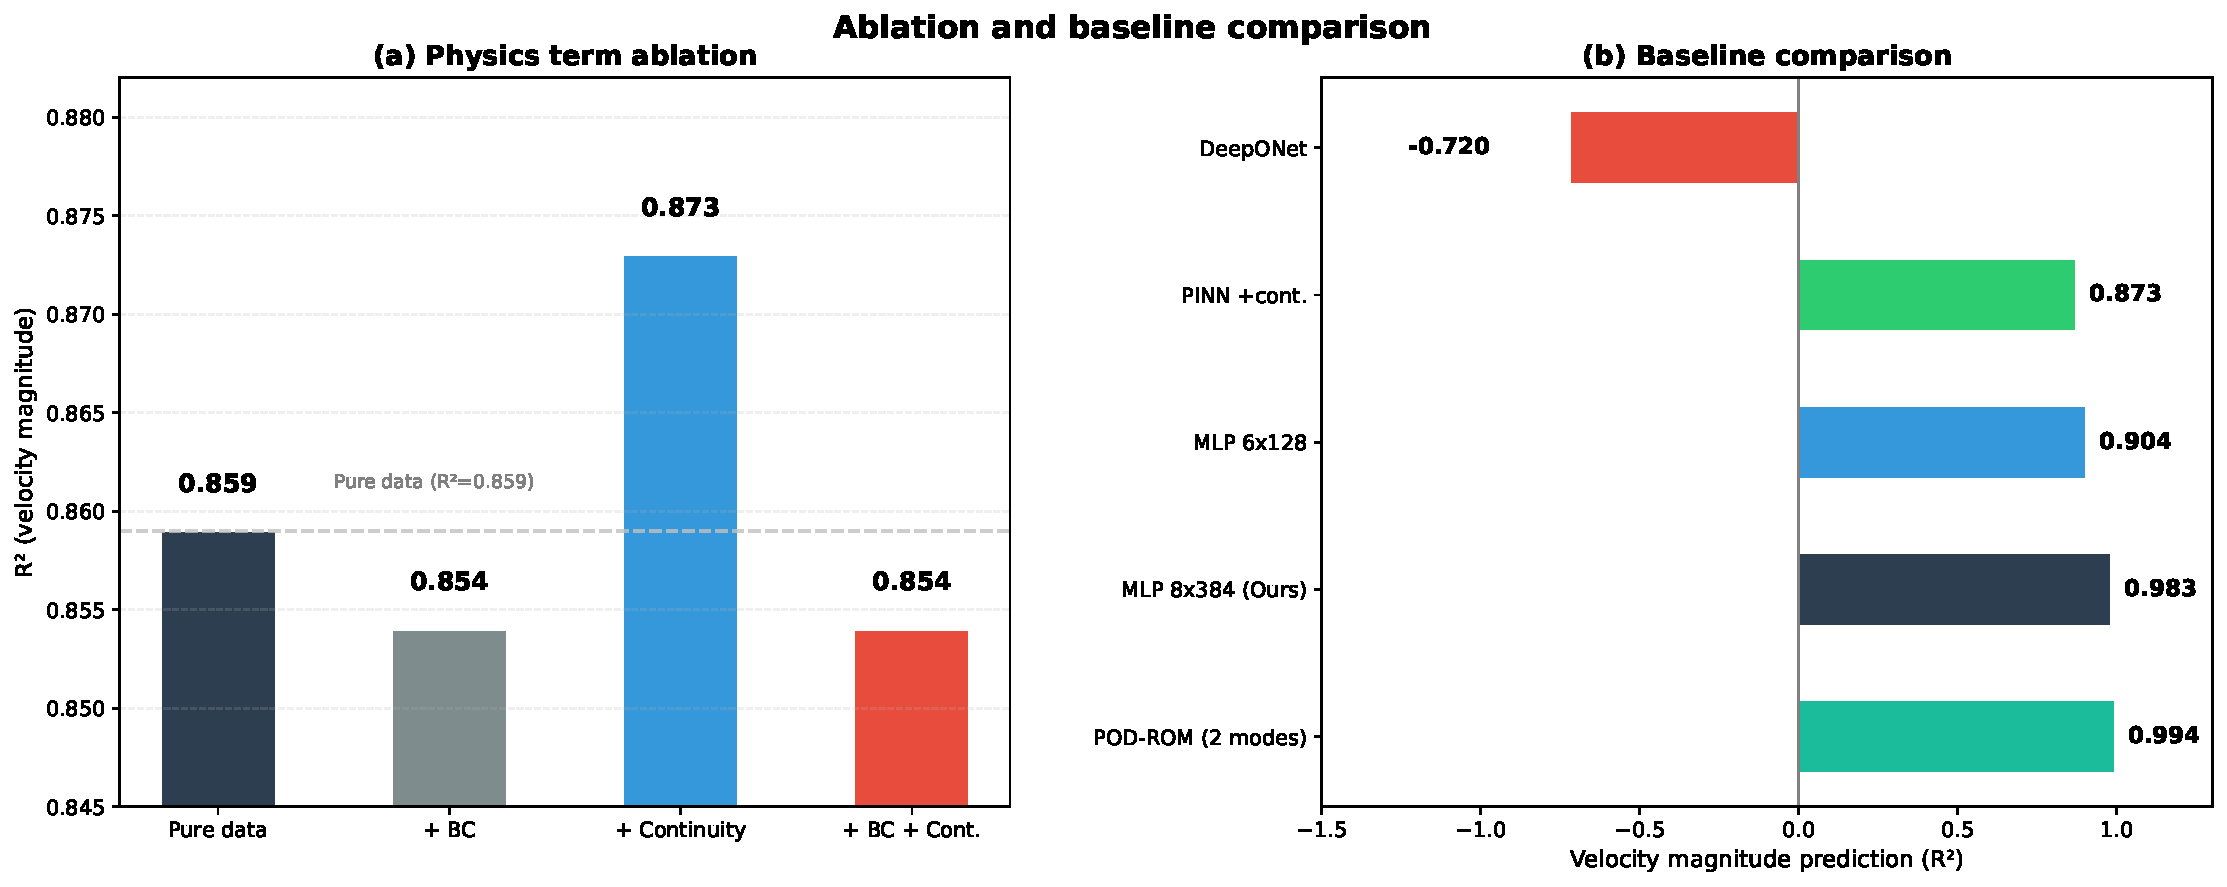
\includegraphics[width=\textwidth]{figures/fig_ablation_baseline.pdf}
\caption{(a) Physics term ablation. (b) Baseline comparison.}
\label{fig:abl_base}
\end{figure}

\subsection{Cross-Position Generalization and POD Limitation}
\label{sec:results_cross}
Cross-position results are shown in Fig.~\ref{fig:cross} and Table~\ref{tab:cross}. A center-only model ($m=0$) collapses on eccentric data ($R^{2}<-0.7$), confirming that injection position fundamentally alters the flow topology. Joint training with $m\in\{0,1\}$ recovers $R^{2}=0.94$--$0.97$ for eccentric cases while maintaining $R^{2}=0.974$ for center-blowing.

Crucially, the center-trained POD model fails catastrophically on eccentric data ($R^{2}=-0.77$ to $-1.40$). This is because POD spatial modes represent the specific spatial structure of the training configuration. Unlike the MLP, POD cannot incorporate a categorical input variable ($m$) to condition its predictions on injection position. Even a ``joint'' POD combining center and eccentric snapshots would produce modes that mix two fundamentally different flow topologies rather than learning to switch between them. Each nozzle configuration therefore requires an independent POD model.

In contrast, the proposed surrogate with $m$ parameterization replaces two separate POD models with a single network. The three-dimensional error comparison (Fig.~\ref{fig:pod}) visualizes this contrast at $Q=120$ NL/min.

\begin{figure}[H]
\centering
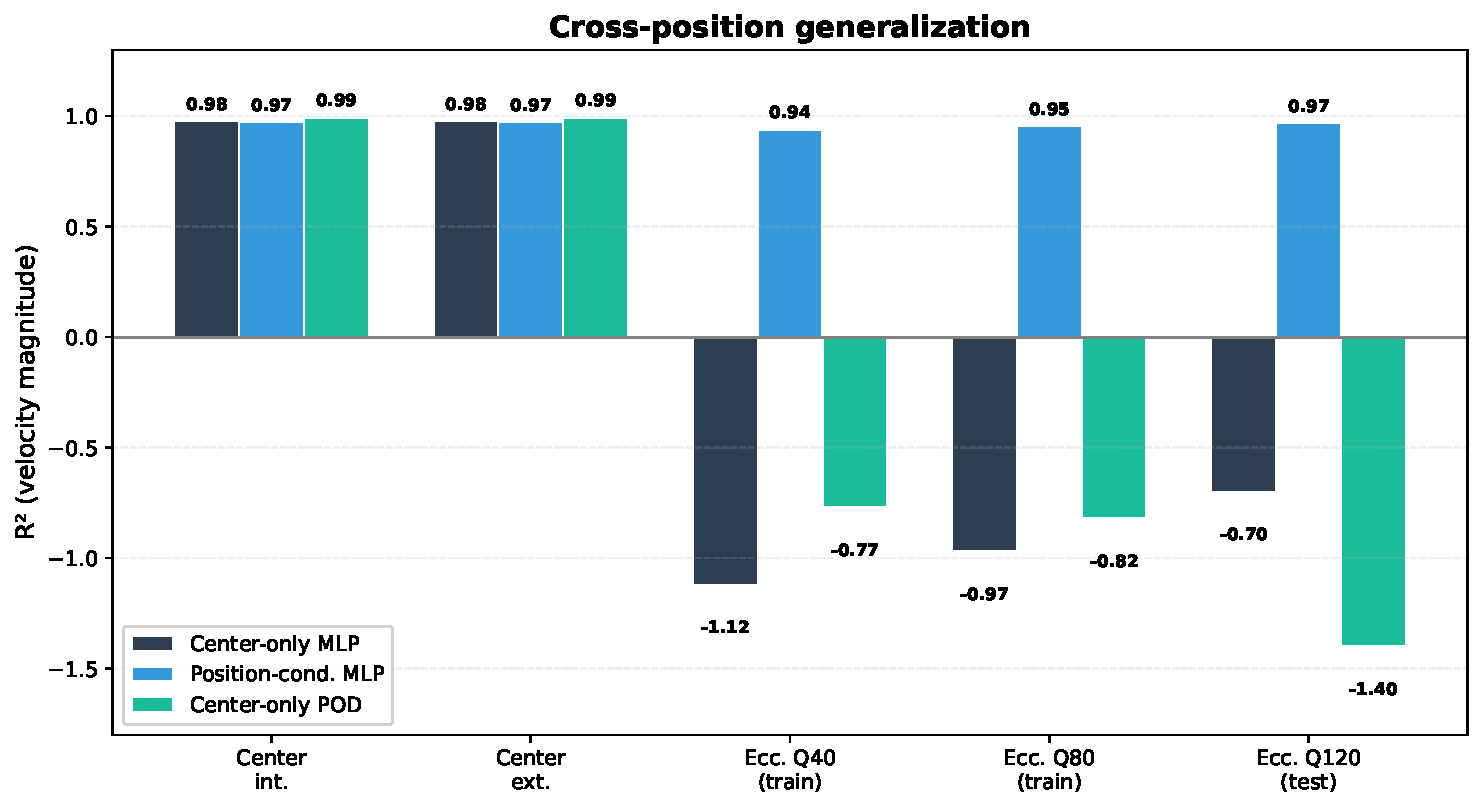
\includegraphics[width=0.95\textwidth]{figures/fig6_cross_position.pdf}
\caption{Cross-position generalization. Center-only models fail; joint model recovers; POD fails catastrophically on eccentric data.}
\label{fig:cross}
\end{figure}

\begin{table}[h]
\centering
\caption{Cross-position generalization.}
\label{tab:cross}
\begin{tabular}{lcccc}
\toprule Model & Center $R^{2}$ & Ecc.\ Q40 & Ecc.\ Q80 & Ecc.\ Q120 \\ \midrule
MLP center-only & 0.979 & $-1.12$ & $-0.97$ & $-0.70$ \\
MLP joint & 0.974 & 0.940 & 0.955 & 0.969 \\
POD center-only & 0.994 & $-0.77$ & $-0.82$ & $-1.40$ \\
\bottomrule
\end{tabular}
\end{table}

\begin{figure}[H]
\centering
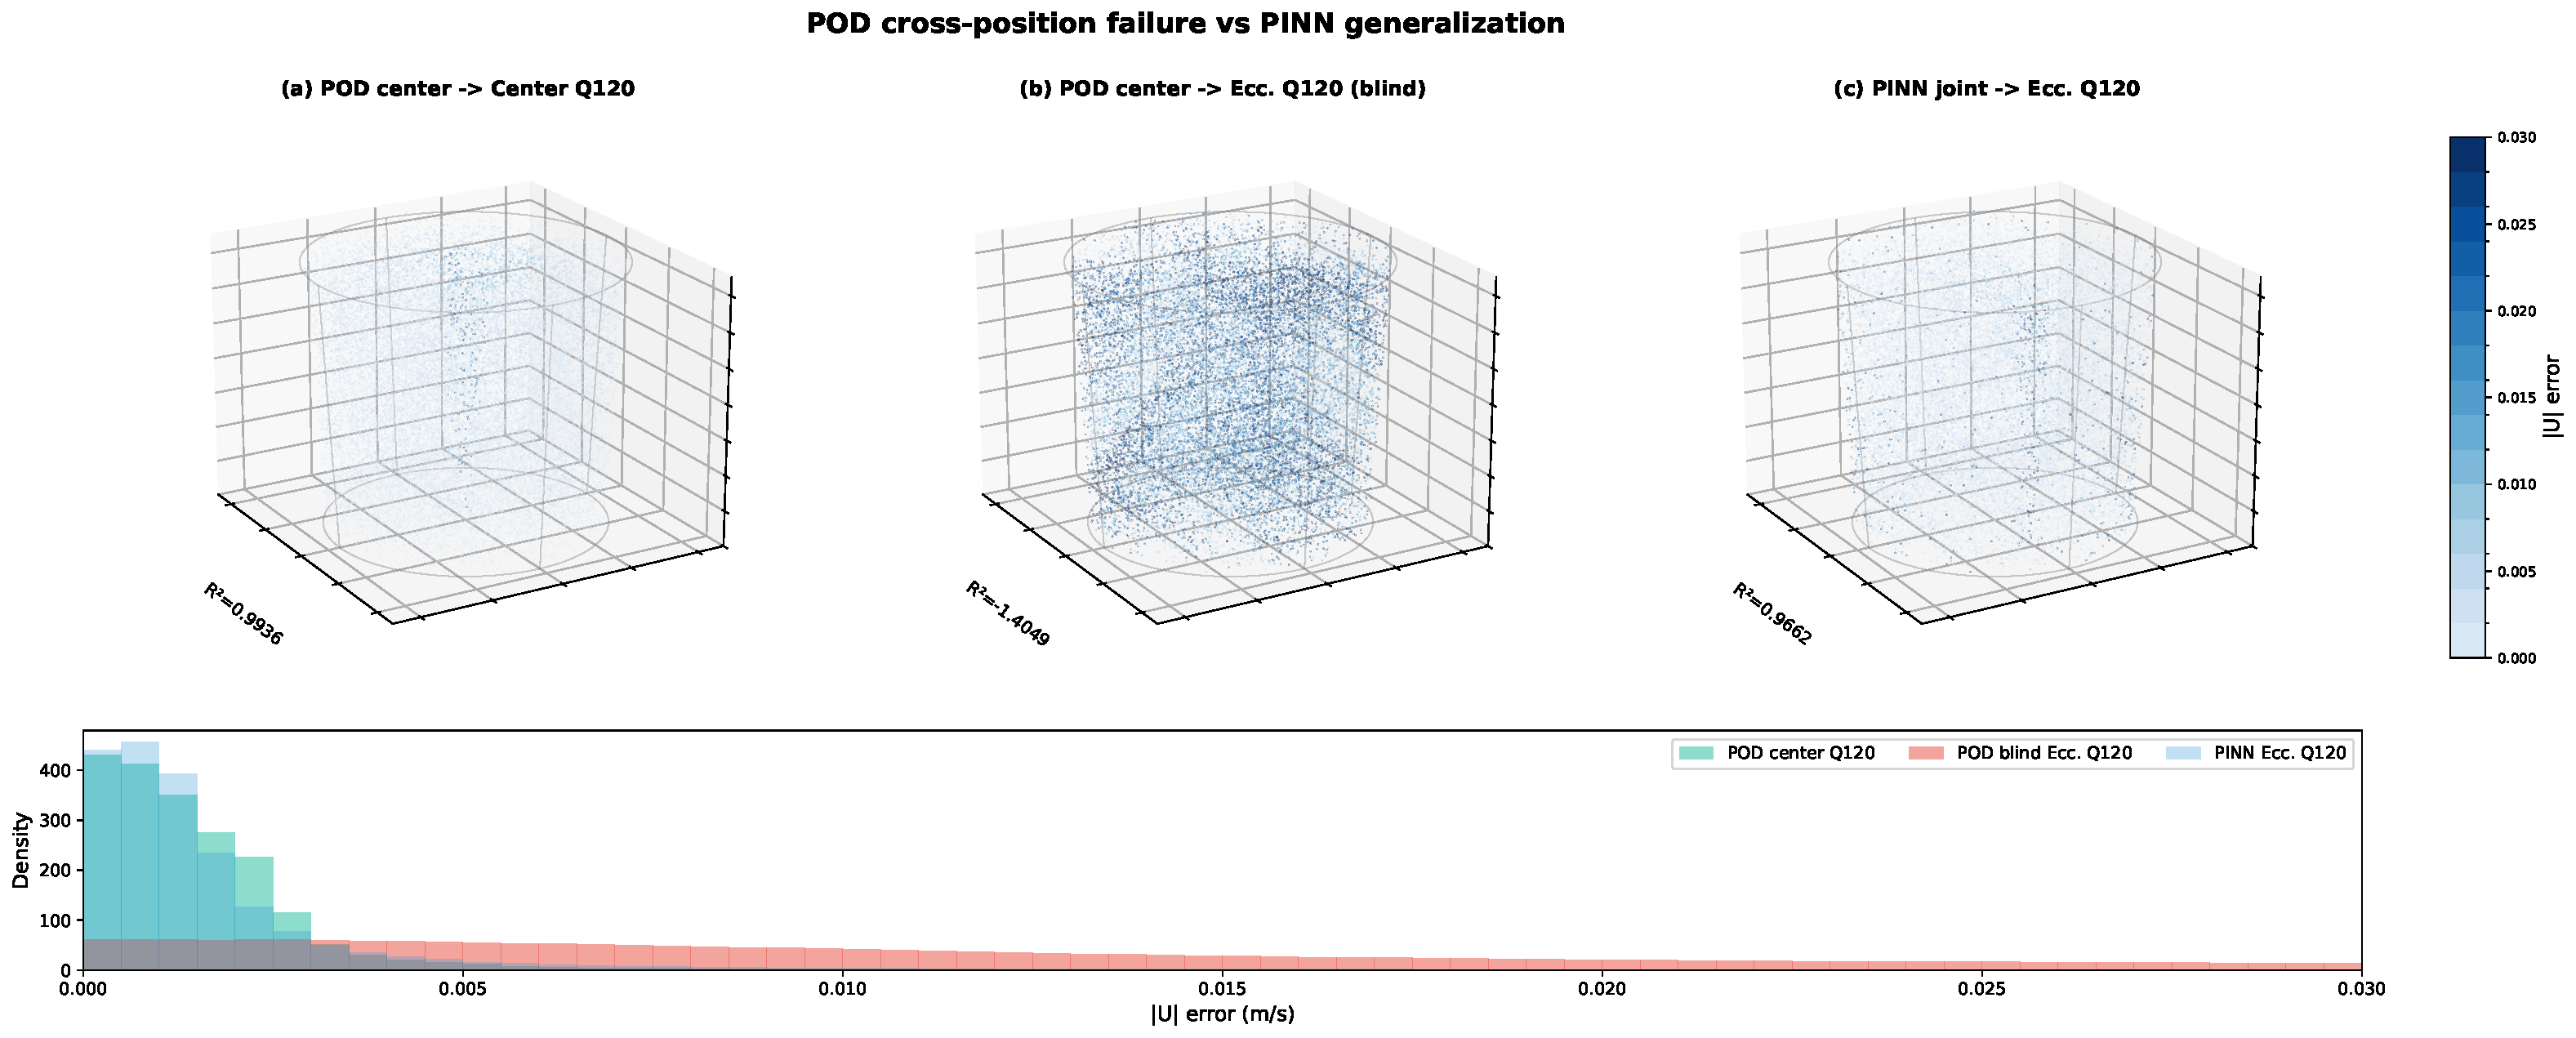
\includegraphics[width=\textwidth]{figures/fig_pod_vs_pinn.pdf}
\caption{POD cross-position failure vs.\ MLP generalization, $Q=120$ NL/min. (a) POD: center-trained, tested on center ($R^{2}=0.994$). (b) Same POD model tested on eccentric data ($R^{2}=-1.40$). (c) Joint MLP on eccentric data ($R^{2}=0.969$). Bottom: error distributions.}
\label{fig:pod}
\end{figure}

\subsection{Pointwise Accuracy and Error Distribution}
Pointwise scatter (Fig.~\ref{fig:scatter}) confirms strong agreement across all conditions. Three-dimensional error visualization (Fig.~\ref{fig:3derror}) shows errors concentrated in the high-gradient plume core. Per-condition performance, multi-seed stability, and VOF sensitivity are summarized in Fig.~\ref{fig:perf}. Training converges smoothly (Fig.~\ref{fig:conv}).

\begin{figure}[H]
\centering
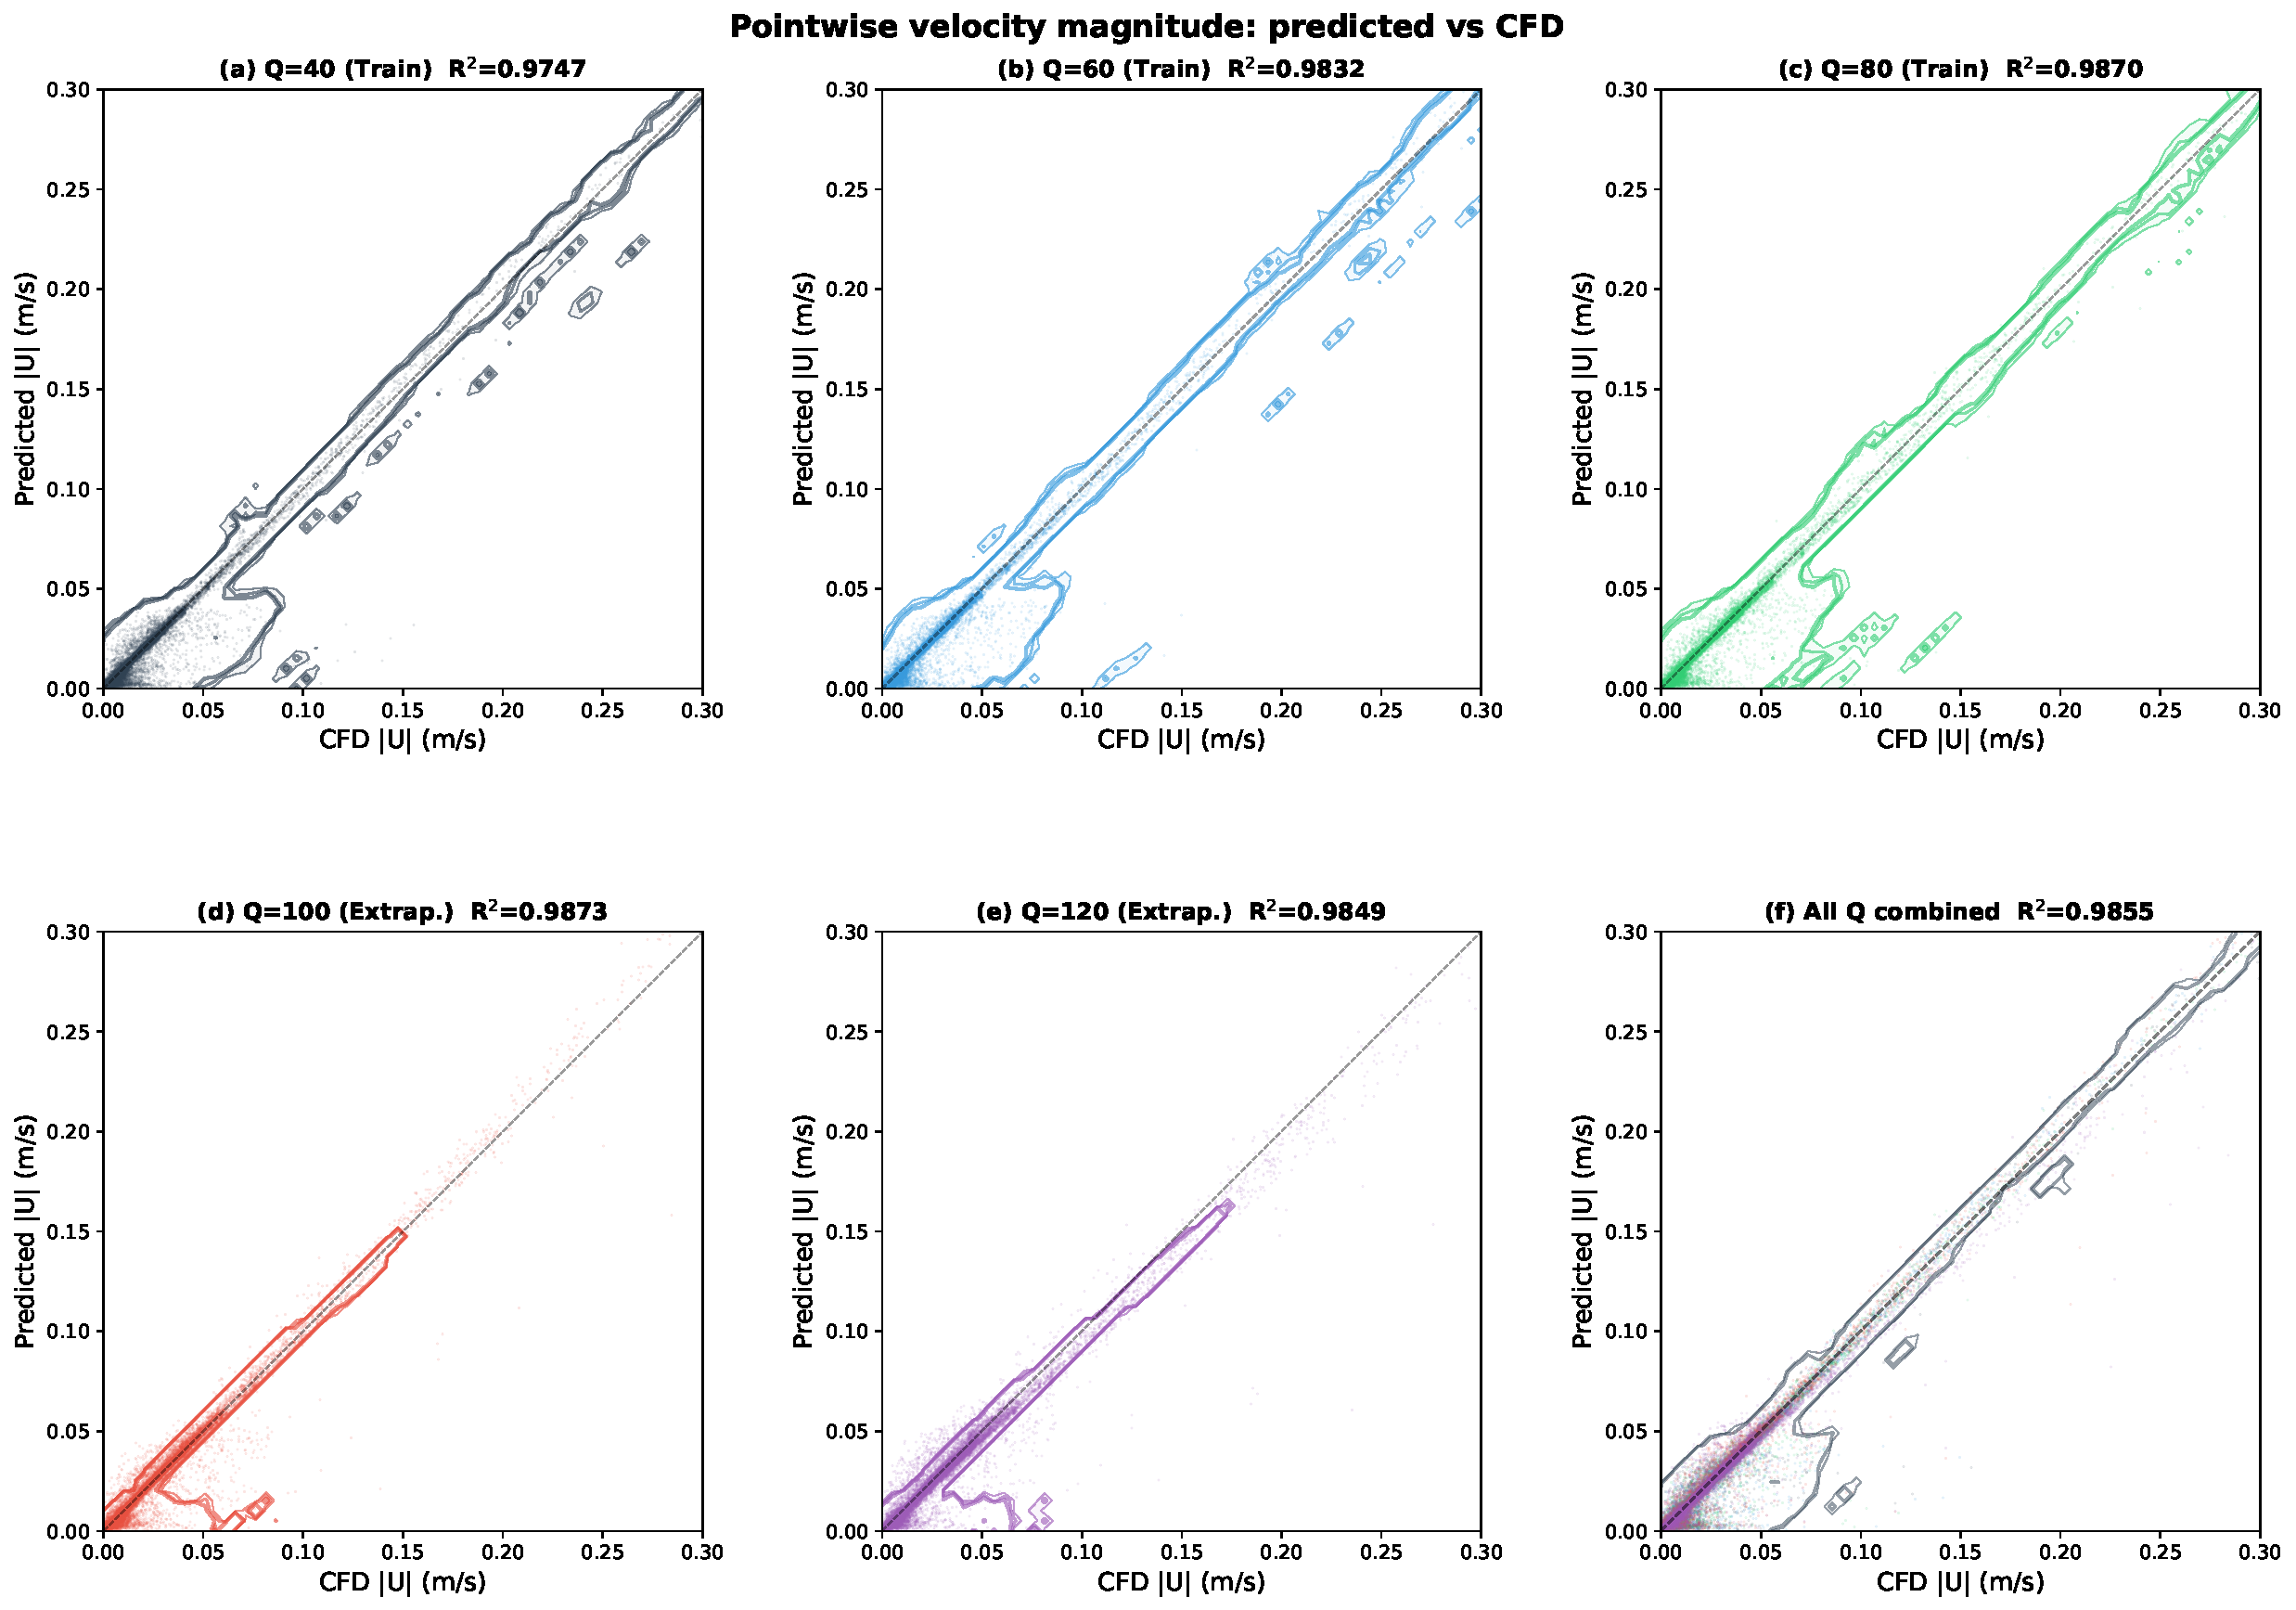
\includegraphics[width=\textwidth]{figures/fig_scatter.pdf}
\caption{Per-condition pointwise comparison. Panels (a--e): individual $Q$. Panel (f): all $Q$ combined.}
\label{fig:scatter}
\end{figure}

\begin{figure}[H]
\centering
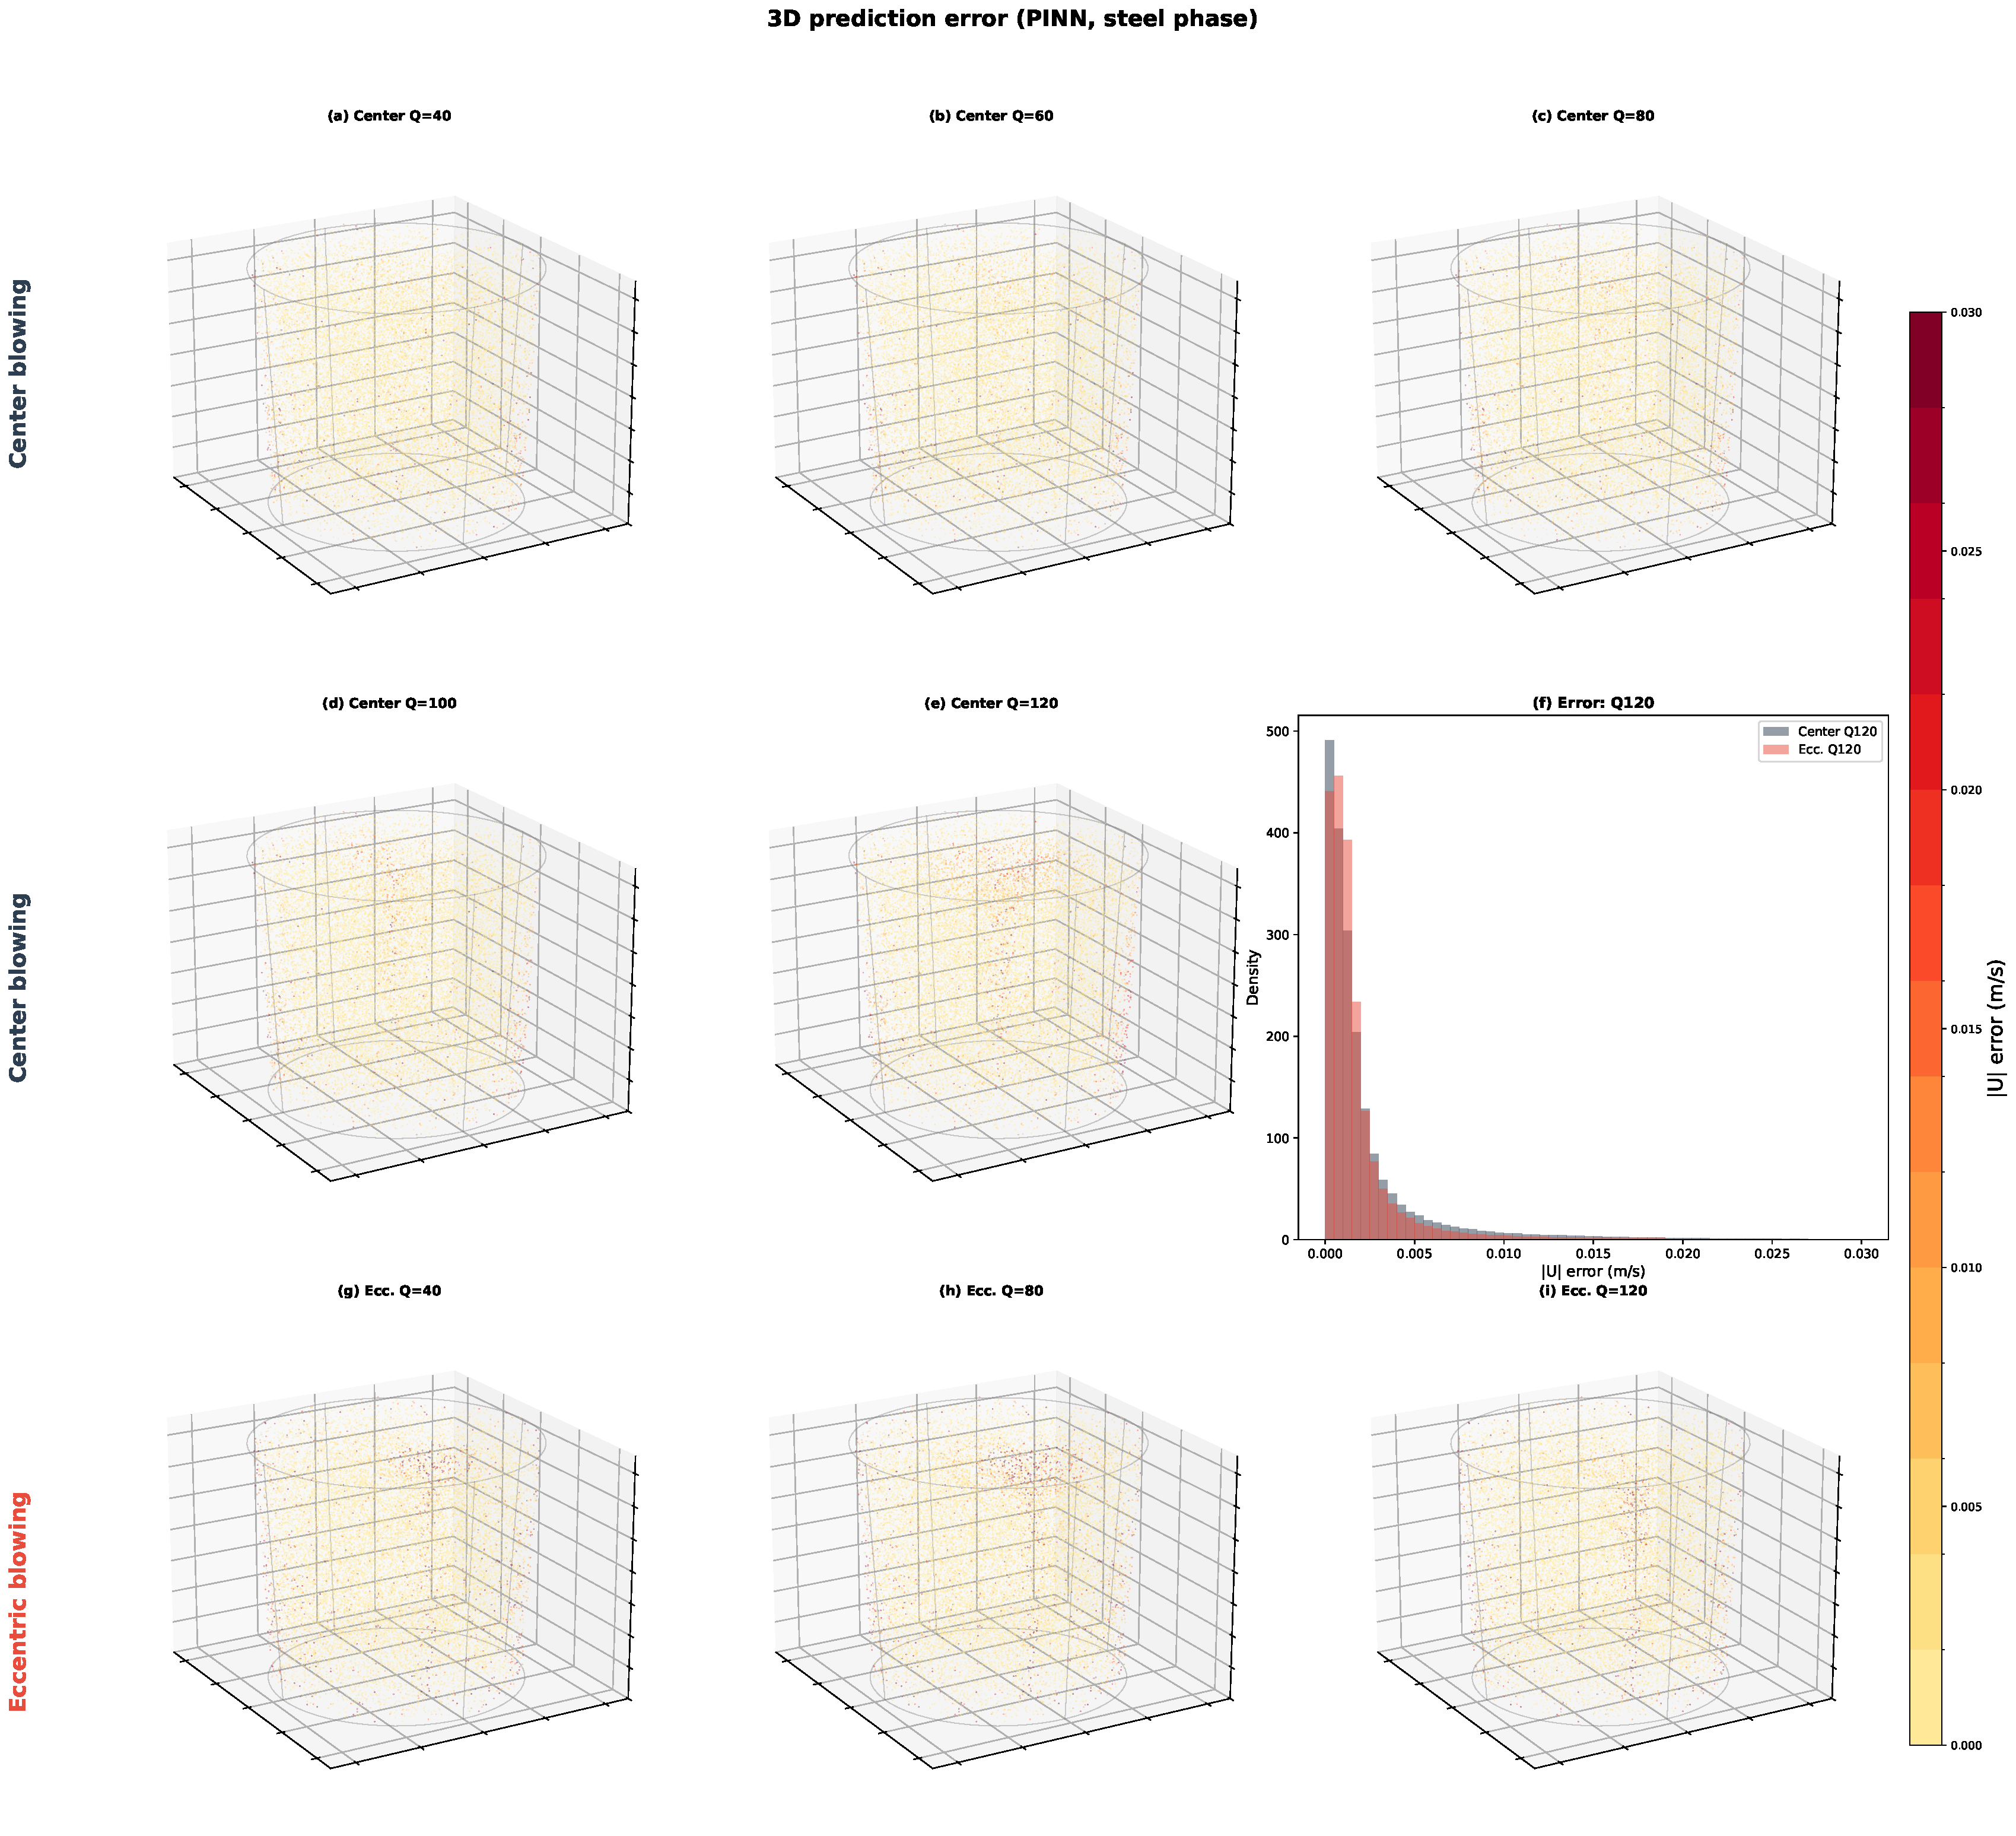
\includegraphics[width=\textwidth]{figures/fig_3d_error.pdf}
\caption{3D prediction error distribution, steel phase. (a--e) Center-blowing. (f) Error histogram. (g--i) Eccentric-blowing.}
\label{fig:3derror}
\end{figure}

\begin{figure}[H]
\centering
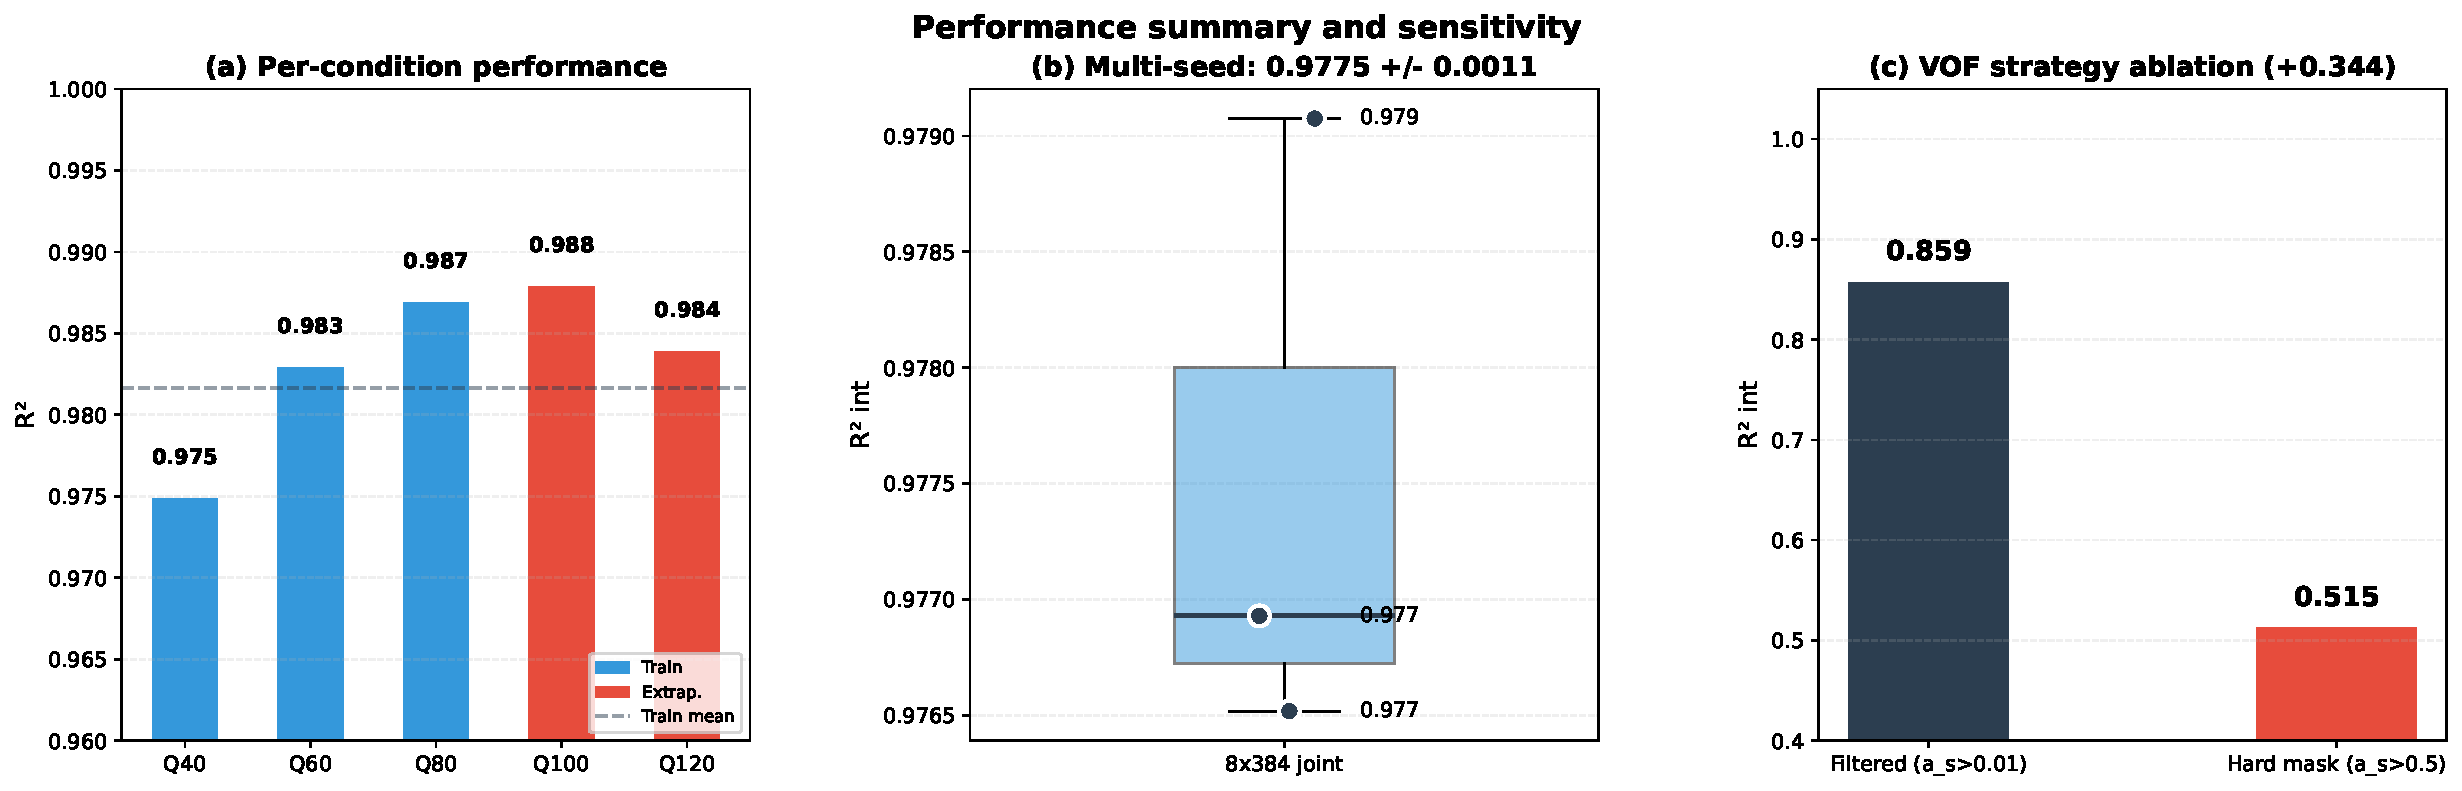
\includegraphics[width=\textwidth]{figures/fig9_performance.pdf}
\caption{(a) Per-condition $R^{2}$. (b) Multi-seed: $0.978\pm0.001$. (c) VOF strategy: filtering vs.\ hard mask.}
\label{fig:perf}
\end{figure}

\begin{figure}[H]
\centering
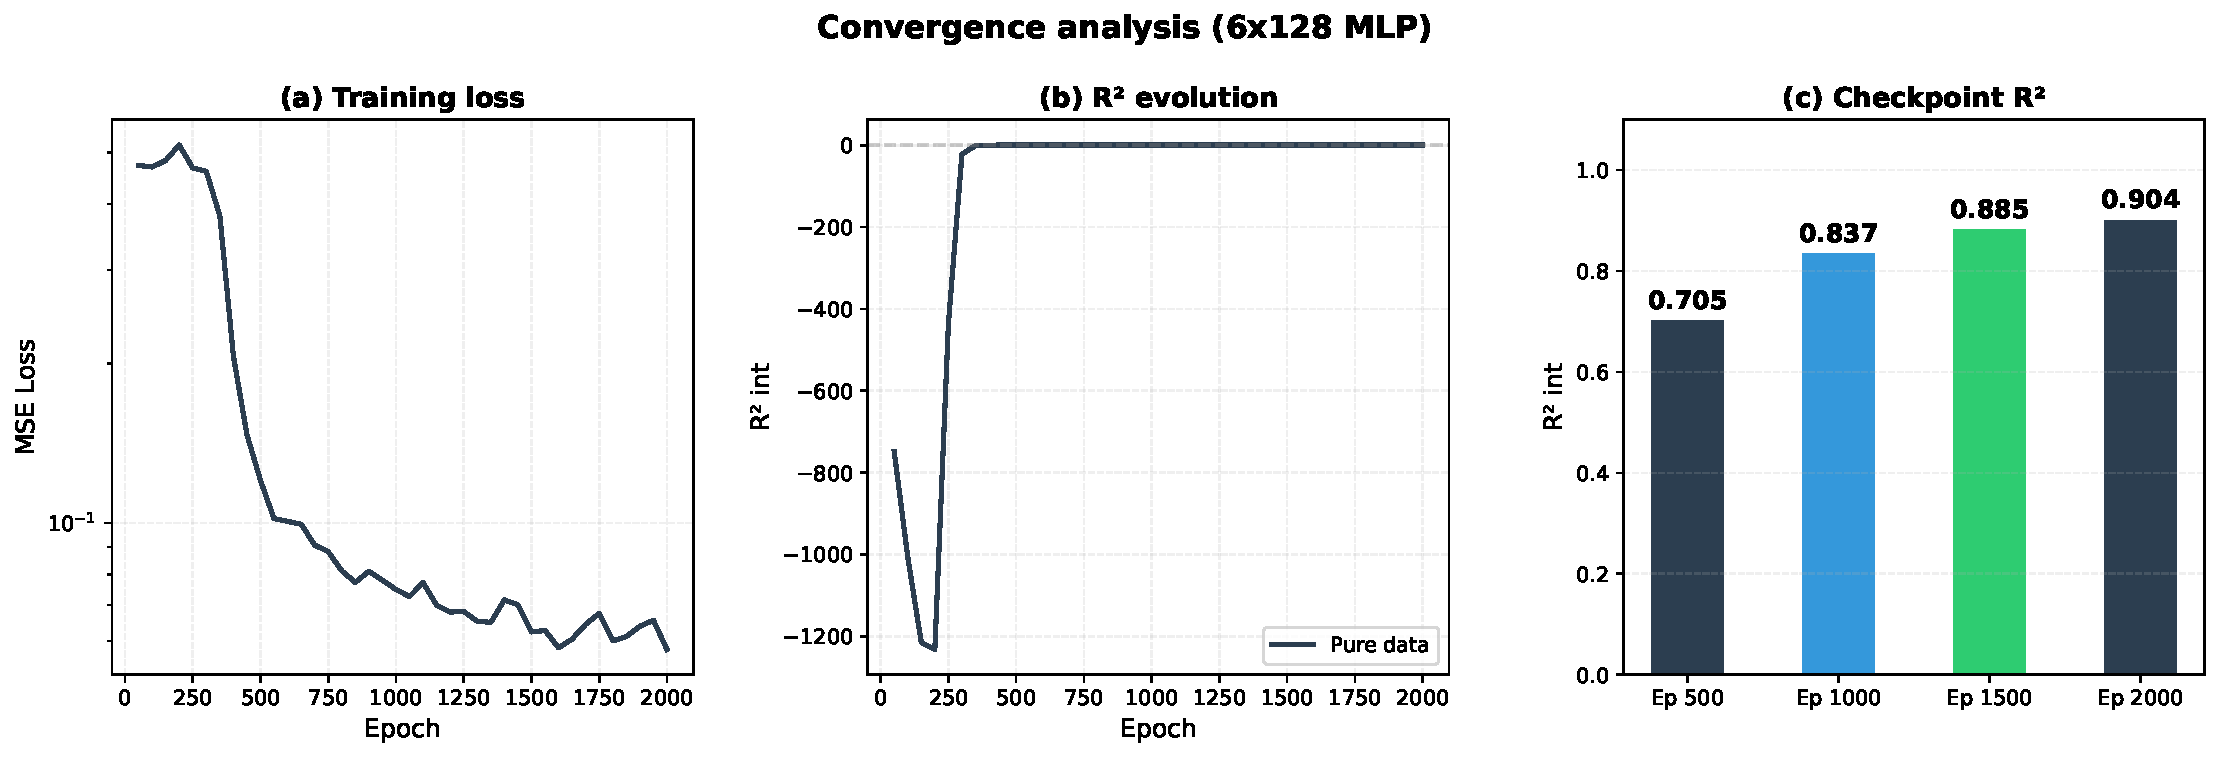
\includegraphics[width=\textwidth]{figures/fig7_convergence.pdf}
\caption{Convergence: (a) training loss, (b) $R^{2}$ evolution, (c) checkpoint values.}
\label{fig:conv}
\end{figure}

\subsection{Three-Dimensional Flow Visualization}
Plume core visualization (Fig.~\ref{fig:3d}) reveals the flow structure. The eccentric plume is offset at $x\approx 0.47$ m, matching the nozzle position.

\begin{figure}[H]
\centering
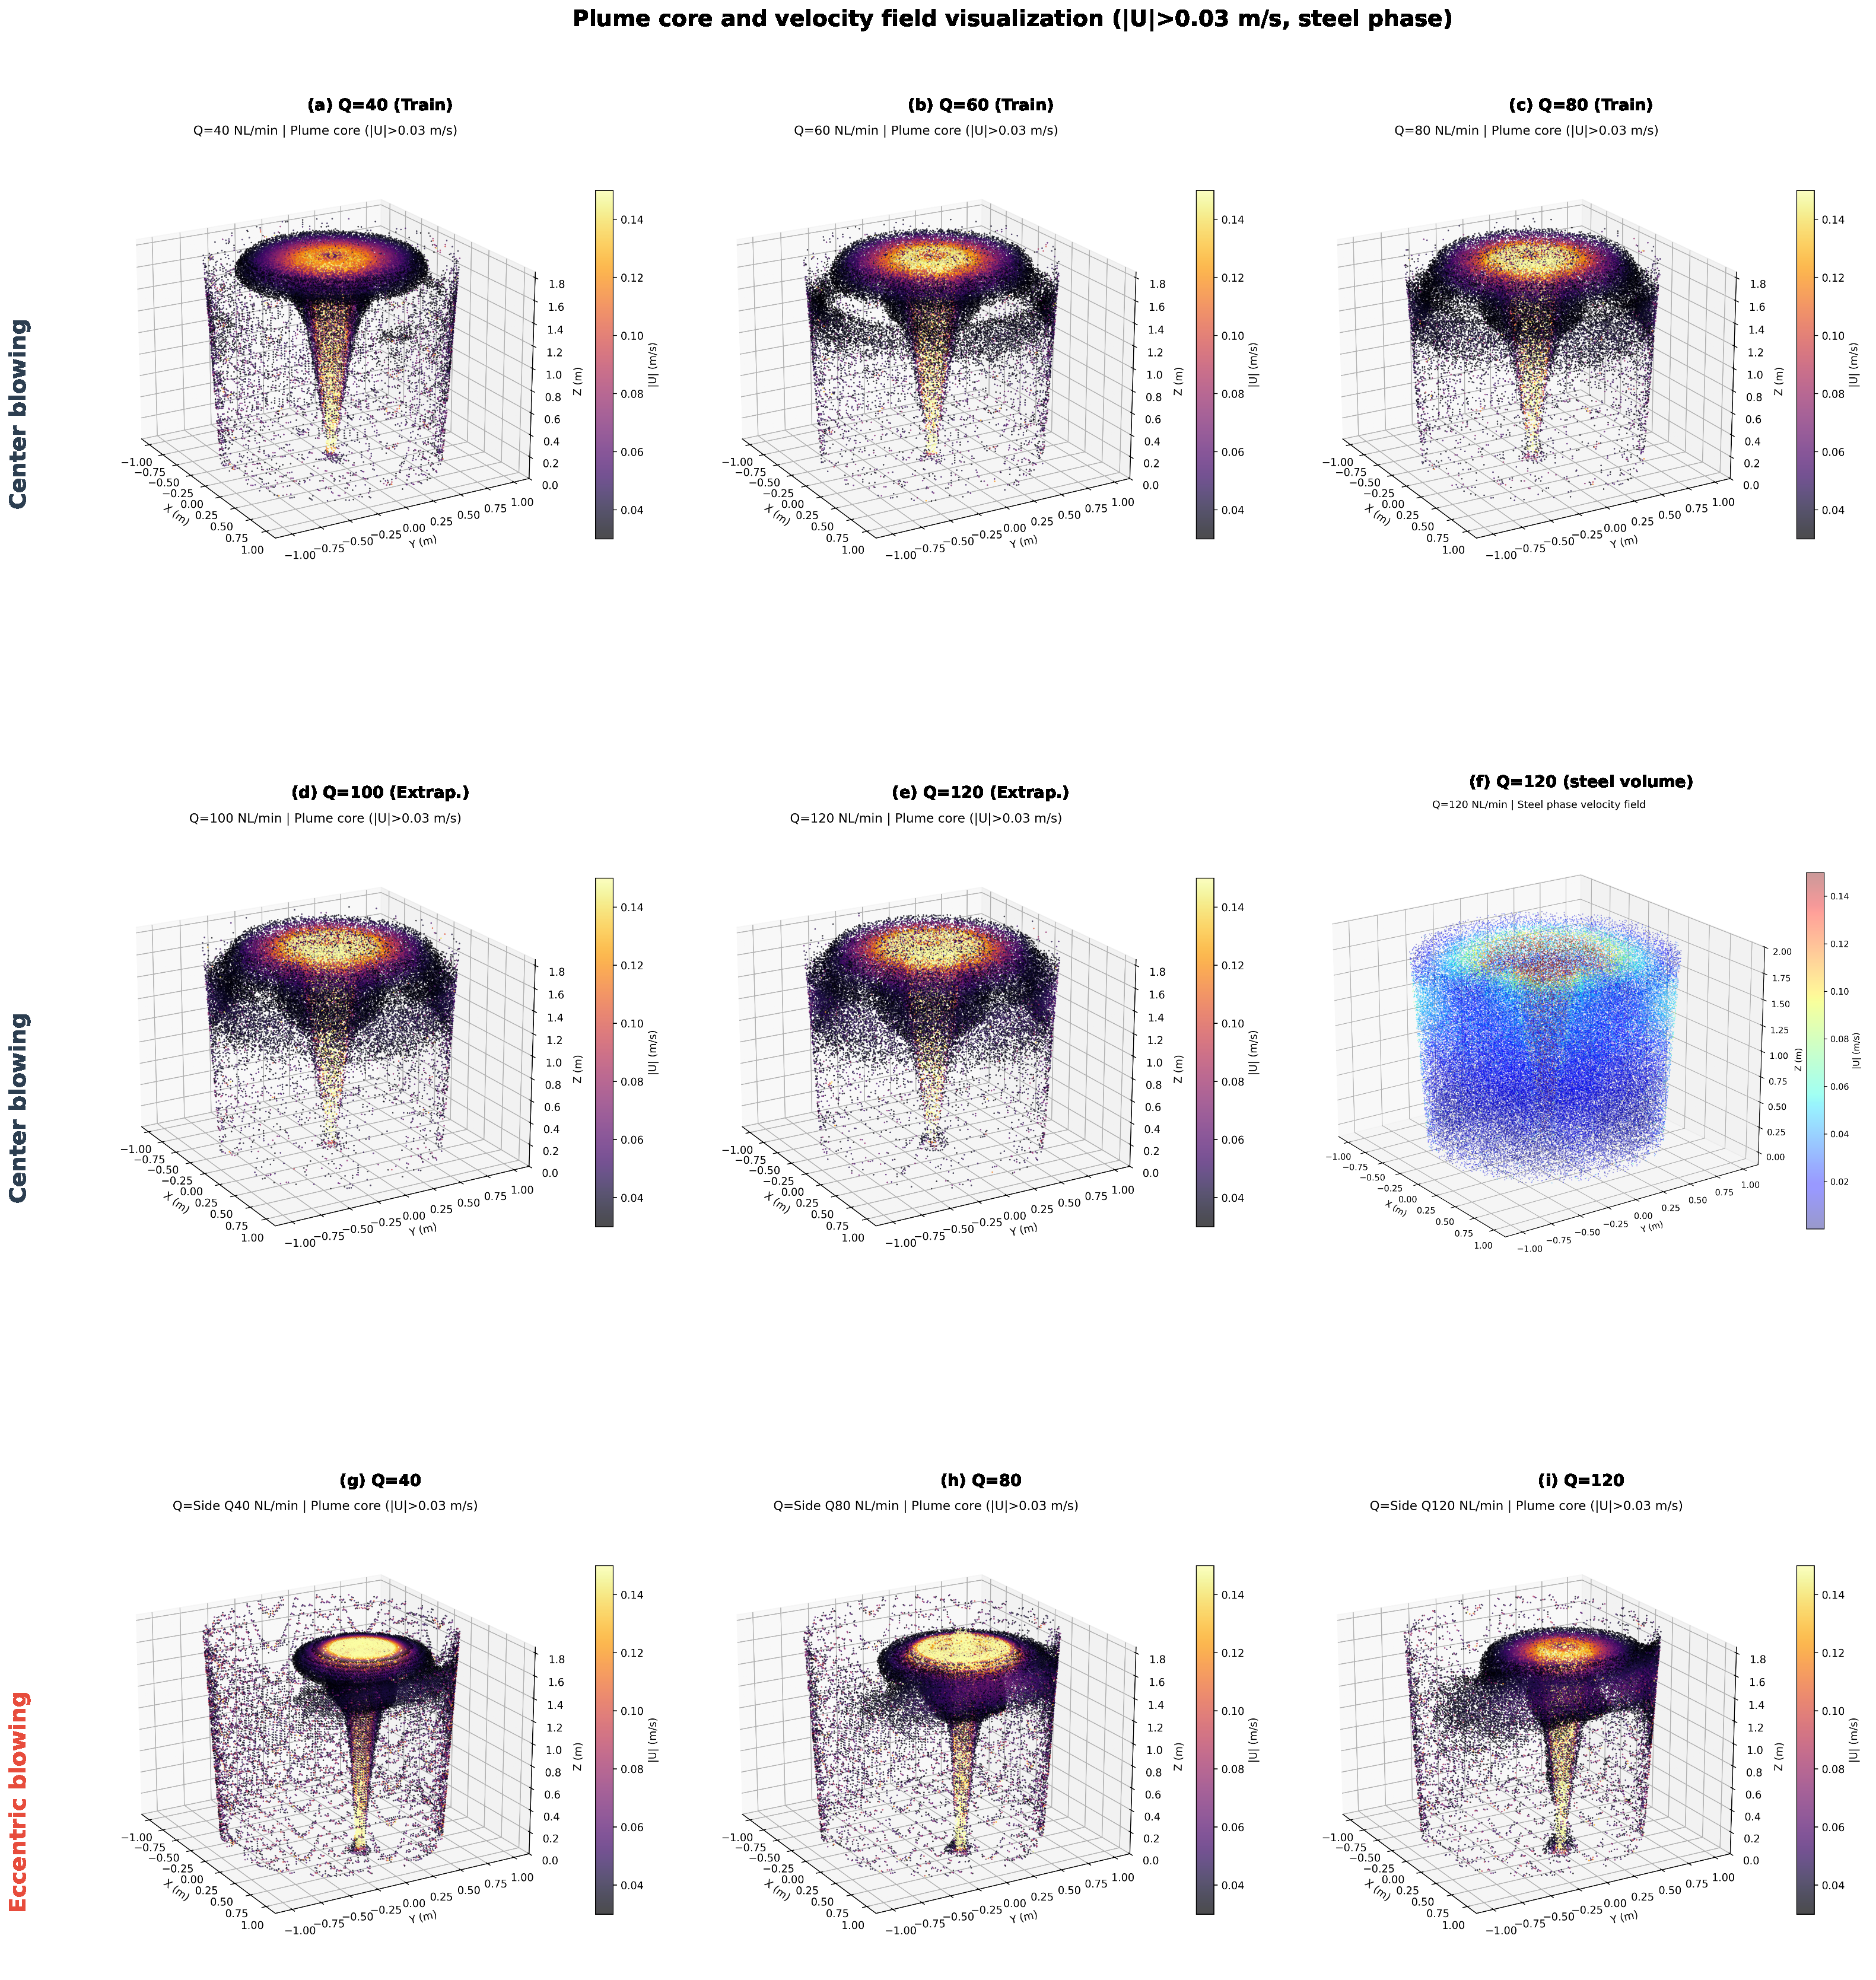
\includegraphics[width=\textwidth]{figures/fig_3d_combined.pdf}
\caption{Plume core ($|\mathbf{U}|>0.03$ m/s). (a--e) Center-blowing. (f) Steel volume. (g--i) Eccentric-blowing.}
\label{fig:3d}
\end{figure}

\FloatBarrier\FloatBarrier
\section{Discussion}

\subsection{Why VOF Filtering Works}
Restricting the problem to the steel phase succeeds for a mathematical reason rather than an empirical one: in pure-steel cells the mixture equations reduce to single-phase RANS without approximation. The filter eliminates the interface region where multiphase momentum balance spans four orders of magnitude, avoiding the ill-conditioning that would plague a full-domain PINN. The soft spatial decay provides a continuous transition, but the dominant effect comes from the filter itself ($+0.344$ $R^{2}$ over hard thresholding; full-domain training collapses).

\subsection{Why POD Outperforms MLP on Center-Blowing}
POD-ROM's center-blowing accuracy ($R^{2}=0.994$) is not an indictment of the MLP but a reflection of problem structure. With three training snapshots, two SVD modes capture all snapshot variance, and thin-plate-spline RBF interpolation of two smoothly varying coefficients yields near-perfect prediction. The MLP ($R^{2}=0.983$) learns a general 5D$\to$4D mapping from a three-point sampling of the $Q$ dimension---a fundamentally harder task. The fact that it approaches POD-level accuracy with such sparse coverage of the parameter space demonstrates the effectiveness of the neural network approach.

\subsection{Why POD Cannot Cross Positions}
POD modes represent the spatial structure of a specific flow configuration. Center-blowing modes capture a centrally symmetric plume; eccentric-blowing requires modes representing an off-center plume. Unlike the MLP, which can learn to condition its output on $m$, POD offers no mechanism for categorical input variables. Even concatenating center and eccentric snapshots into a joint POD would blend two incompatible spatial patterns rather than learning to switch between them. The MLP's $m$ parameterization enables a single model to serve both configurations---replacing two independent POD models with one network.

\subsection{Physics Regularization: When It Helps}
The continuity constraint provides a consistent but small gain ($+0.014$ $R^{2}$) for the $6\times128$ model, where limited capacity benefits from additional guidance. For the $8\times384$ model, pure data supervision is sufficient. The momentum residual does not help regardless of model size because the DPM bubble buoyancy---the actual plume driver---is absent from the homogeneous RANS formulation. BC constraints are unnecessary because the no-slip condition is implicitly encoded in the CFD data. These findings suggest that for CFD-informed surrogate problems where training data are dense and noise-free, physics regularization offers diminishing returns as model capacity increases.

\subsection{Limitations}
(1) Steady-state only---transient slag eye dynamics require time-resolved training. (2) No explicit bubble physics in the surrogate---DPM momentum is encoded in CFD data, not in the model. (3) Single ladle geometry. (4) Three training $Q$ values---the zero extrapolation degradation suggests this is sufficient for the studied range, but outer bounds remain untested. (5) Kriging, POD (cross-position), and KAN encountered implementation barriers that limit the completeness of the baseline comparison. Future work will extend this framework in three directions: (1) time-resolved CFD training data to capture transient slag eye opening and closing dynamics, (2) structural feature extraction from plume-induced flow patterns (e.g., recirculation zone topology, interface deformation metrics) as inputs to downstream prediction models, and (3) a coupled inclusion transport and removal-rate prediction model built on the surrogate flow field---combining the high-throughput CFD-DPM data-generation framework of the companion study \cite{liu2026cfd} with the rapid surrogate inference demonstrated here.

\FloatBarrier\section{Conclusion}
A CFD-informed surrogate using VOF-based domain decomposition and an $8\times384$ SiLU MLP achieves $R^{2}=0.983$ for center-blowing with near-zero extrapolation degradation. Joint $m\in\{0,1\}$ training recovers $R^{2}=0.94$--$0.97$ for eccentric-blowing. Six baselines were compared. POD-ROM achieves the best center-blowing accuracy ($R^{2}=0.994$) but collapses across injection positions because spatial modes do not transfer between configurations---each position requires an independent POD model. The proposed surrogate with $m$ parameterization replaces two POD models with one network, predicting the full field in $\sim$5 seconds.

\section*{Acknowledgments}
Supported by National Key R\&D Program of China (2023YFB3712401).

\section*{Data Availability}
The CFD-DPM simulation code used to generate the reference dataset is available at \texttt{https://github.com/YimLiu626/-ladle-cfd-bucket-screening} \cite{liu2026cfd}. All surrogate modeling code, trained model weights, result JSON files, and paper figures are available at \texttt{https://github.com/YimLiu626/ladle-pinn-surrogate}. A sample of the 12-column CFD export format (100 rows) is included in the surrogate repository.

\bibliographystyle{elsarticle-num}
\begin{thebibliography}{99}

\bibitem{liu2026cfd} Liu Y., Wu G. A cell-localized bucket search method for conservative bubble-inclusion contact screening in industrial CFD-DPM simulations. \textit{Advances in Manufacturing}, 2026 (under review).

\bibitem{mazumdar1995physical} Mazumdar D., Guthrie R.I.L. The physical and mathematical modelling of gas stirred ladle systems. \textit{ISIJ International}, 1995, 35(1): 1--20.

\bibitem{jonsson1996modeling} Jonsson L., J\"{o}nsson P. Modeling of fluid flow conditions around the slag/metal interface in a gas-stirred ladle. \textit{ISIJ International}, 1996, 36(9): 1127--1134.

\bibitem{li2020numerical} Li L., Li X., Zhu Z., et al. Numerical modeling of multiphase flow in gas-stirred ladles: A review. \textit{Powder Technology}, 2020, 373: 14--25.

\bibitem{xin2024modeling} Xin Z., Zhang J., Peng K., et al. Modeling of LF refining process: A review. \textit{J. Iron Steel Res. Int.}, 2024, 31: 289--317.

\bibitem{liu2019numerical} Liu Y., Ersson M., Liu H., et al. A review of physical and numerical approaches for gas stirring in ladle metallurgy. \textit{Metall. Mater. Trans. B}, 2019, 50: 555--577.

\bibitem{ersson2008fluid} Ersson M., Tilliander A., Jonsson L., et al. A mathematical model of an impinging air jet on a water surface. \textit{ISIJ International}, 2008, 48(4): 377--384.

\bibitem{brunton2020machine} Brunton S.L., Noack B.R., Koumoutsakos P. Machine learning for fluid mechanics. \textit{Annu. Rev. Fluid Mech.}, 2020, 52: 477--508.

\bibitem{raissi2019physics} Raissi M., Perdikaris P., Karniadakis G.E. Physics-informed neural networks. \textit{J. Comput. Phys.}, 2019, 378: 686--707.

\bibitem{karniadakis2021physics} Karniadakis G.E., Kevrekidis I.G., Lu L., et al. Physics-informed machine learning. \textit{Nature Rev. Phys.}, 2021, 3: 422--440.

\bibitem{cai2021physics} Cai S., Mao Z., Wang Z., et al. PINNs for fluid mechanics: A review. \textit{Acta Mech. Sinica}, 2021, 37: 1727--1738.

\bibitem{cuomo2022scientific} Cuomo S., Di Cola V.S., Giampaolo F., et al. Scientific machine learning through PINNs. \textit{J. Sci. Comput.}, 2022, 92(3): 88.

\bibitem{wang2021understanding} Wang S., Teng Y., Perdikaris P. Understanding gradient flow pathologies in PINNs. \textit{SIAM J. Sci. Comput.}, 2021, 43(5): A3055--A3081.

\bibitem{jin2021nsfnet} Jin X., Cai S., Li H., et al. NSFnets. \textit{J. Comput. Phys.}, 2021, 426: 109951.

\bibitem{shih1995new} Shih T.H., et al. A new $k$--$\varepsilon$ eddy viscosity model. \textit{Comput. Fluids}, 1995, 24(3): 227--238.

\bibitem{cloete2010mathematical} Cloete S.W.P., et al. Fluid flow and mixing in full-scale gas-stirred ladles. \textit{Prog. Comput. Fluid Dyn.}, 2009, 9(6--7): 345--356.

\bibitem{benner2015survey} Benner P., Gugercin S., Willcox K. A survey of projection-based model reduction methods. \textit{SIAM Review}, 2015, 57(4): 483--531.

\bibitem{lu2021deeponet} Lu L., Jin P., Pang G., et al. Learning nonlinear operators via DeepONet. \textit{Nature Mach. Intell.}, 2021, 3: 218--229.

\bibitem{liu2024kan} Liu Z., Wang Y., Vaidya S., et al. KAN: Kolmogorov--Arnold Networks. \textit{arXiv preprint arXiv:2404.19756}, 2024.

\bibitem{williams2006gaussian} Williams C.K.I., Rasmussen C.E. \textit{Gaussian Processes for Machine Learning}. MIT Press, 2006.

\bibitem{iguchi1995water} Iguchi M., Nakamura K., Tsujino R. Water model experiment on the behavior of gas jets and plumes in a molten metal bath. \textit{ISIJ International}, 1995, 35(3): 224--231.

\bibitem{sahai1996melt} Sahai Y., Emi T. Melt flow characterization in continuous casting tundishes. \textit{ISIJ International}, 1996, 36(6): 667--672.

\bibitem{zhu2019physics} Zhu Y., Zabaras N., Koutsourelakis P.S., Perdikaris P. Physics-constrained deep learning for high-dimensional surrogate modeling. \textit{J. Comput. Phys.}, 2019, 394: 56--81.

\bibitem{sun2020surrogate} Sun L., Gao H., Pan S., Wang J.X. Surrogate modeling for fluid flows based on physics-constrained deep learning without simulation data. \textit{Comput. Methods Appl. Mech. Eng.}, 2020, 361: 112732.

\bibitem{raissi2019hidden} Raissi M., Wang Z., Triantafyllou M.S., Karniadakis G.E. Hidden fluid mechanics: Learning velocity and pressure fields from flow visualizations. \textit{Science}, 2020, 367(6481): 1026--1030.

\bibitem{kaiss2023synth} Kaiss H., Zabaras N. Synthesizing high-fidelity CFD simulation data for surrogate modeling using physics-informed generative models. \textit{Comput. Methods Appl. Mech. Eng.}, 2023, 409: 115956.

\bibitem{berkooz1993pod} Berkooz G., Holmes P., Lumley J.L. The proper orthogonal decomposition in the analysis of turbulent flows. \textit{Annu. Rev. Fluid Mech.}, 1993, 25: 539--575.

\bibitem{launder1974numerical} Launder B.E., Spalding D.B. The numerical computation of turbulent flows. \textit{Comput. Methods Appl. Mech. Eng.}, 1974, 3(2): 269--289.

\bibitem{chattopadhyay2010physical} Chattopadhyay K., Isac M., Guthrie R.I.L. Physical and mathematical modelling of steelmaking tundish operations: A review. \textit{ISIJ International}, 2010, 50(3): 331--348.

\bibitem{conejo2015optimization} Conejo A.N., Hernandez D.E. Optimization of fluid flow in shrouded hot metal mixers. \textit{ISIJ International}, 2015, 55(7): 1347--1355.

\end{thebibliography}

\end{document}
